%----------------------------------------------------------------------------------------
%	PACKAGES AND THEMES
%----------------------------------------------------------------------------------------
\documentclass[aspectratio=169,xcolor=dvipsnames]{beamer}
\usetheme{SimplePlus}

\usepackage{hyperref}
\usepackage{graphicx} % Allows including images
\usepackage{booktabs} % Allows the use of \toprule, \midrule and \bottomrule in tables

%----------------------------------------------------------------------------------------
%	TITLE PAGE
%----------------------------------------------------------------------------------------

\title{NuScenes Based Tracking Project Status Report} % The short title appears at the bottom of every slide, the full title is only on the title page

\date{\today} % Date, can be changed to a custom date


%----------------------------------------------------------------------------------------
%	PRESENTATION SLIDES
%----------------------------------------------------------------------------------------

\begin{document}

\begin{frame}
    % Print the title page as the first slide
    \titlepage
\end{frame}

%------------------------------------------------
%------------------------------------------------
\begin{frame}{Experiment Result}
    \href{https://docs.google.com/spreadsheets/d/e/2PACX-1vQg2MSCst4ShlC0e7T_lr_q4azo-DfDo53On89BjeisHAKJrggMLoTUxcvurpXomLZilYKoWmMMf6U4/pubhtml}{\beamergotobutton{result}}
\end{frame}

\begin{frame}{implementation details for improved score}
    \begin{itemize}
        \item{tracking based on classification instead of tracking with all measurements}
        \item{"label" for id. Previously, we used GNN for generate id, but here we used label.}
    \end{itemize}
\end{frame}

\begin{frame}{how to label}
    \begin{itemize}
        \item{step one, if the max id is 0, means it has not been assigned a label yet. Then for each measurement which turns into bernouli component, assign a label by its measurement index }
        \item{}
    \end{itemize}
\end{frame}

\begin{frame}{Key Issue}
    \begin{itemize}
        \item{false negative (missed track)}
        \begin{itemize}
            \item{Reason 1 slow to initiate a track. It usually takes 2-5 steps to start a track. }
            \item{Reason 2 when there is occlution, restart a track resulting in false negative. One of the key issue related to false negative is occlution. The detection might not be robust, or non-existance. Restart a track will waste valuable frame time. }
        \end{itemize}
        \item{advantage: less false positive, compare to other methods. They would initiate a track right away, regardless if that measurement is a clutter. Our approach is the 'wait and see' methods.}
    \end{itemize}
\end{frame}

\begin{frame}{How Do I know?}
    \begin{itemize}
        \item{Observing the estimated state, step by step. The break point is set at estimated state, then every step i observe the estimated step.}
        \item{Visualization. Generate the BEV of the tracking result. See demo. }
    \end{itemize}
\end{frame}

\begin{frame}{Demo}
        \begin{figure}
            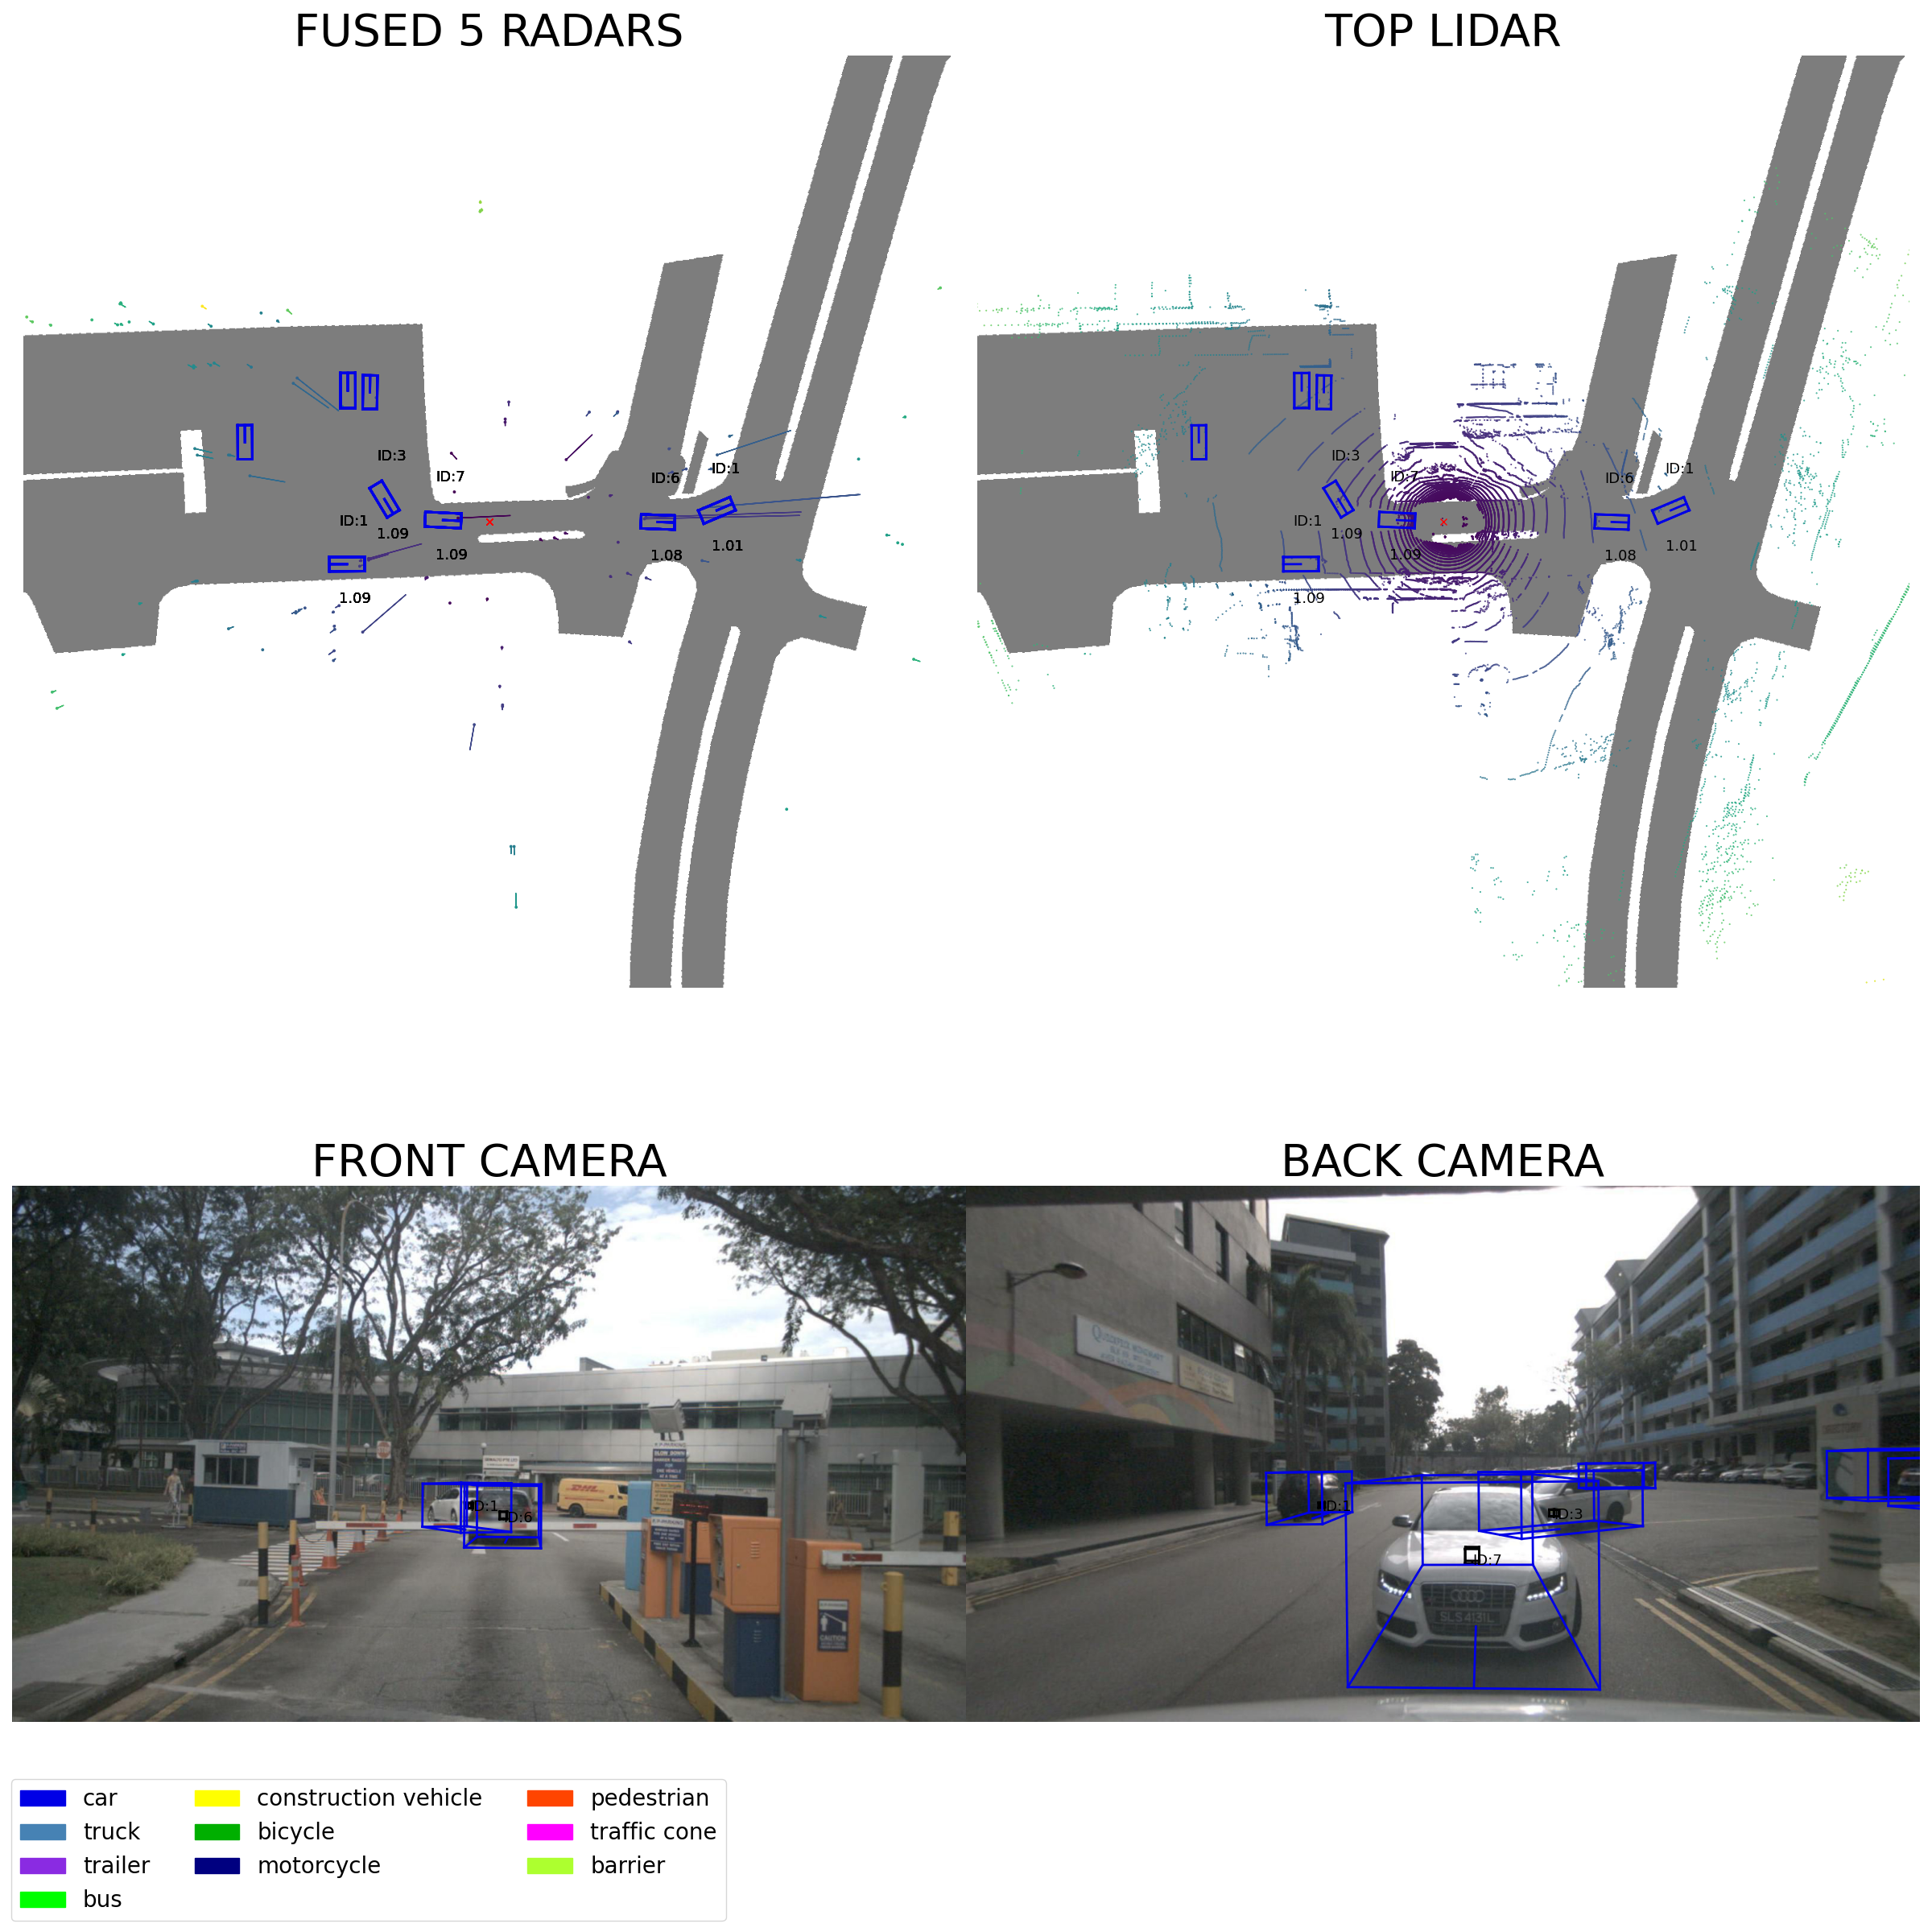
\includegraphics[width=0.4\linewidth]{demo/17.png}
        \end{figure}
\end{frame}
\begin{frame}{Demo}
    \begin{figure}
        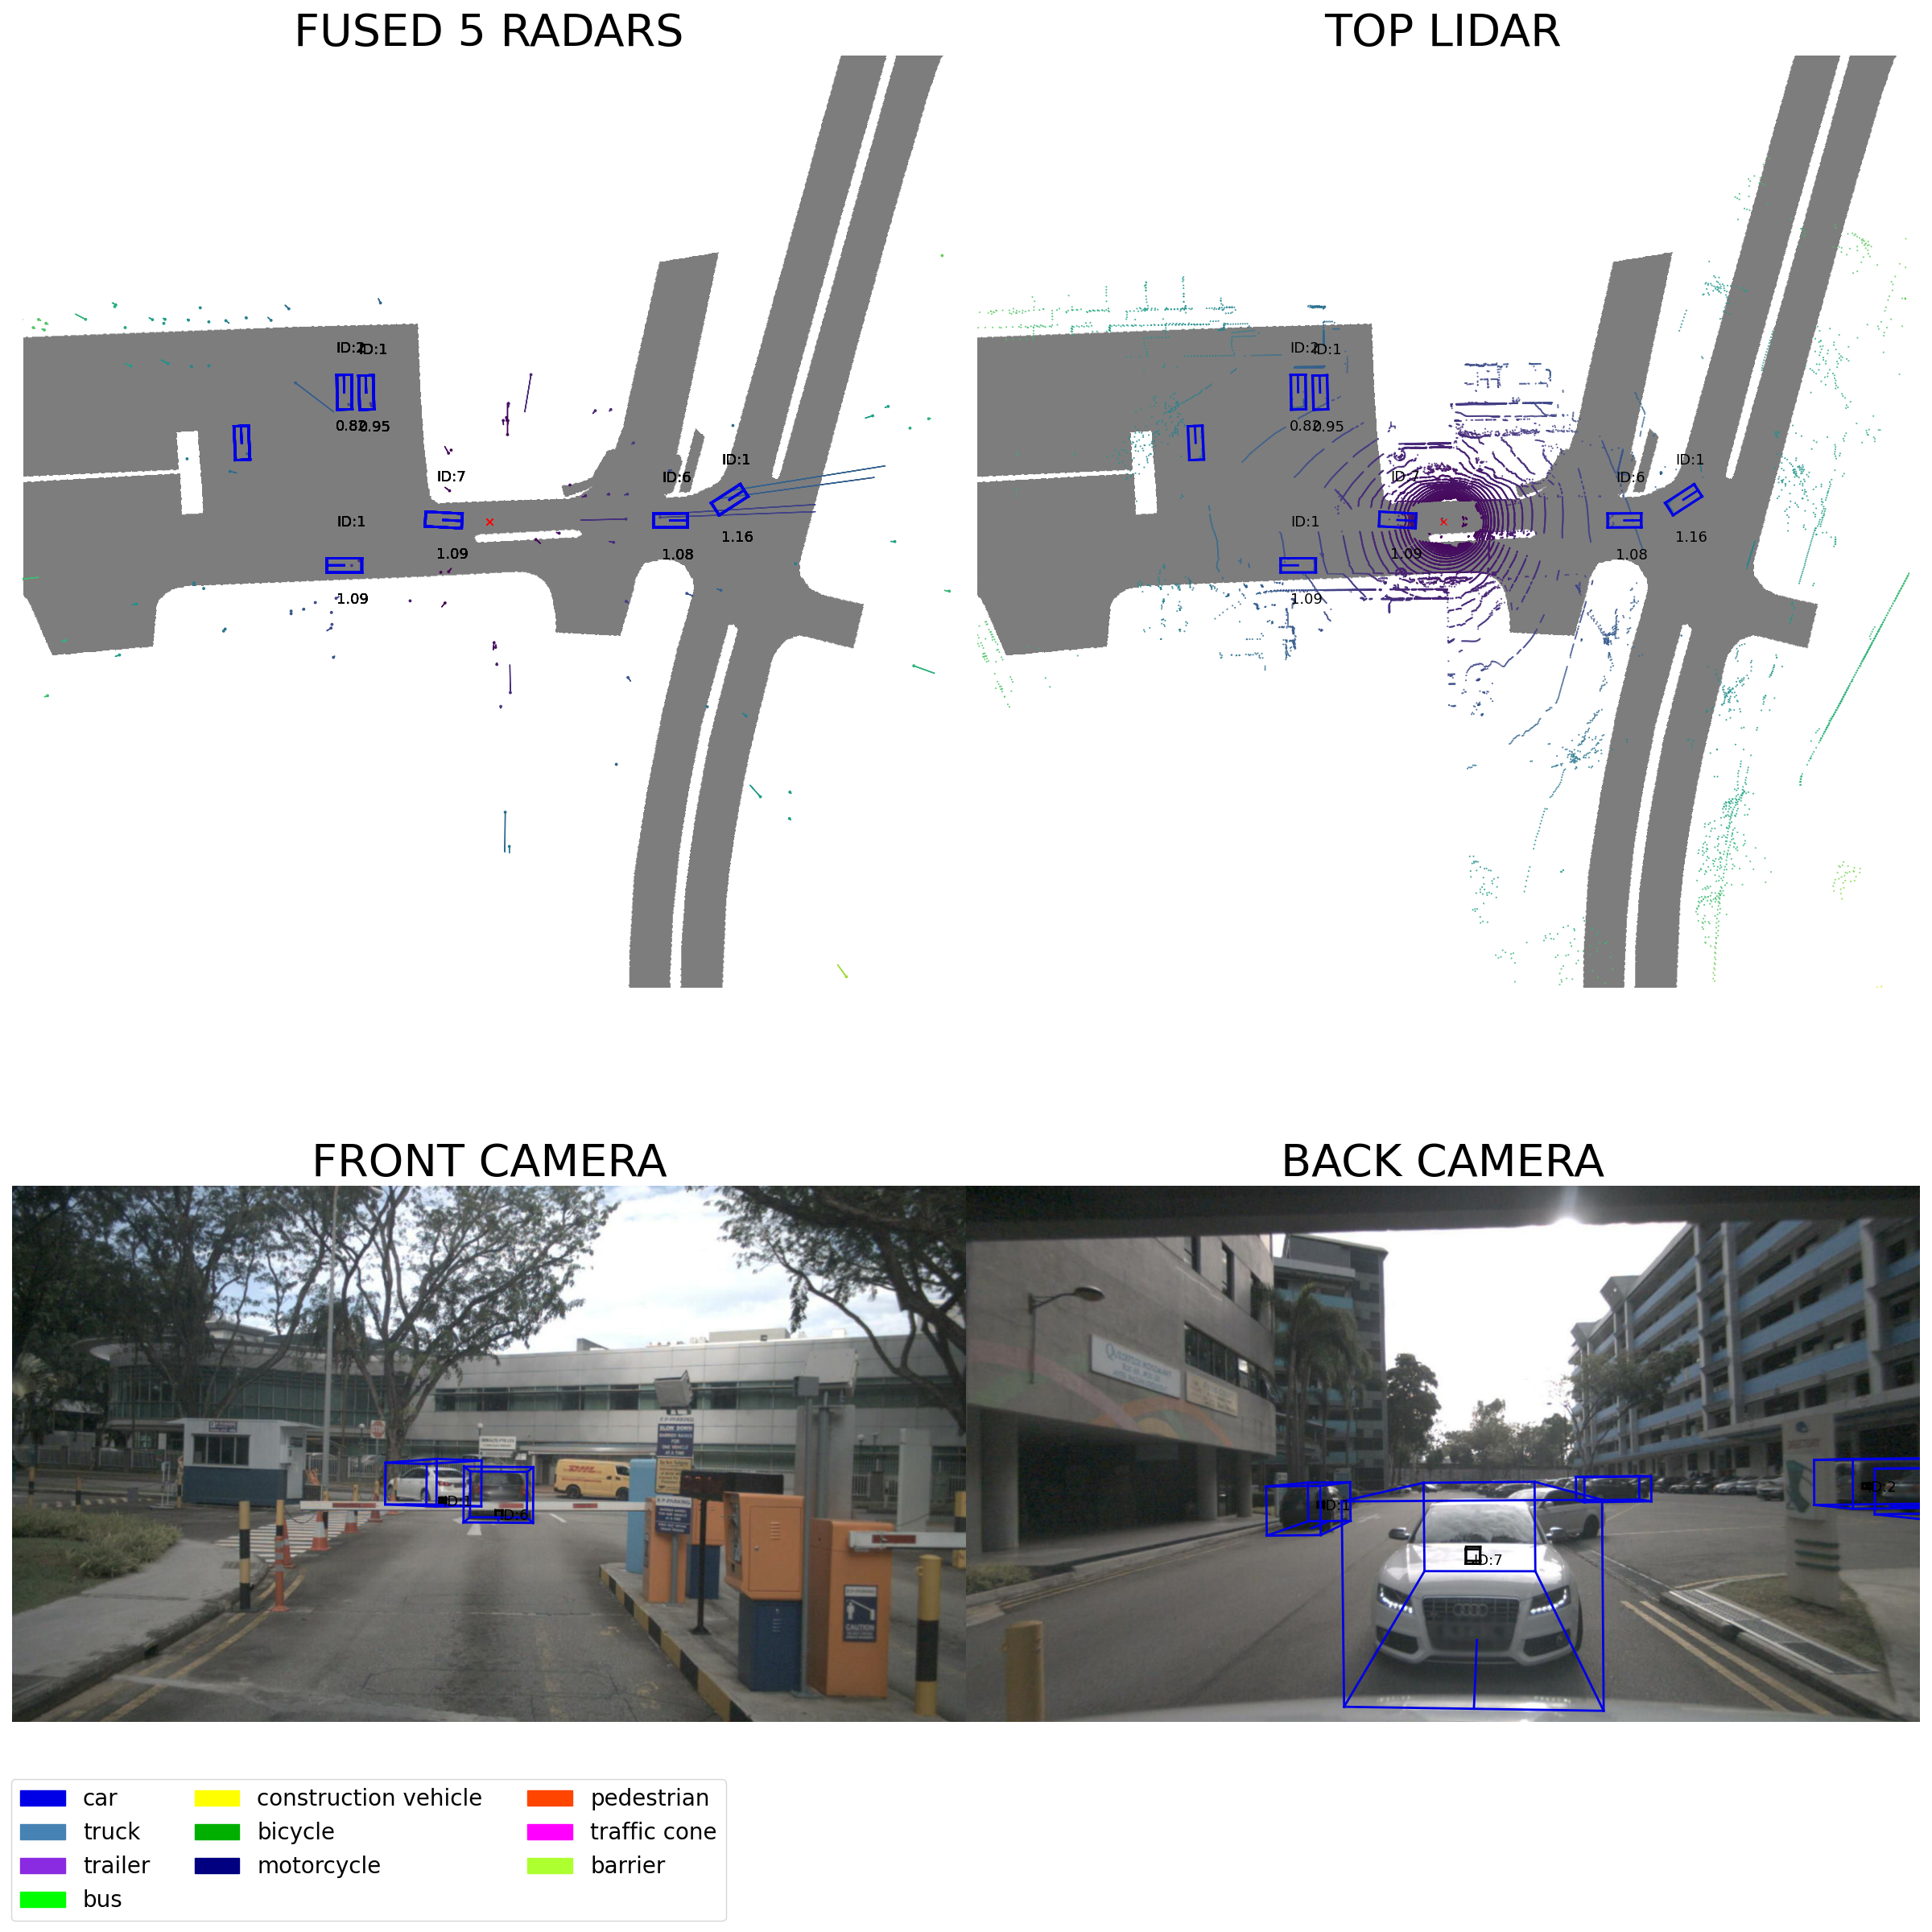
\includegraphics[width=0.4\linewidth]{demo/18.png}
    \end{figure}
\end{frame}
\begin{frame}{Demo}
    \begin{figure}
        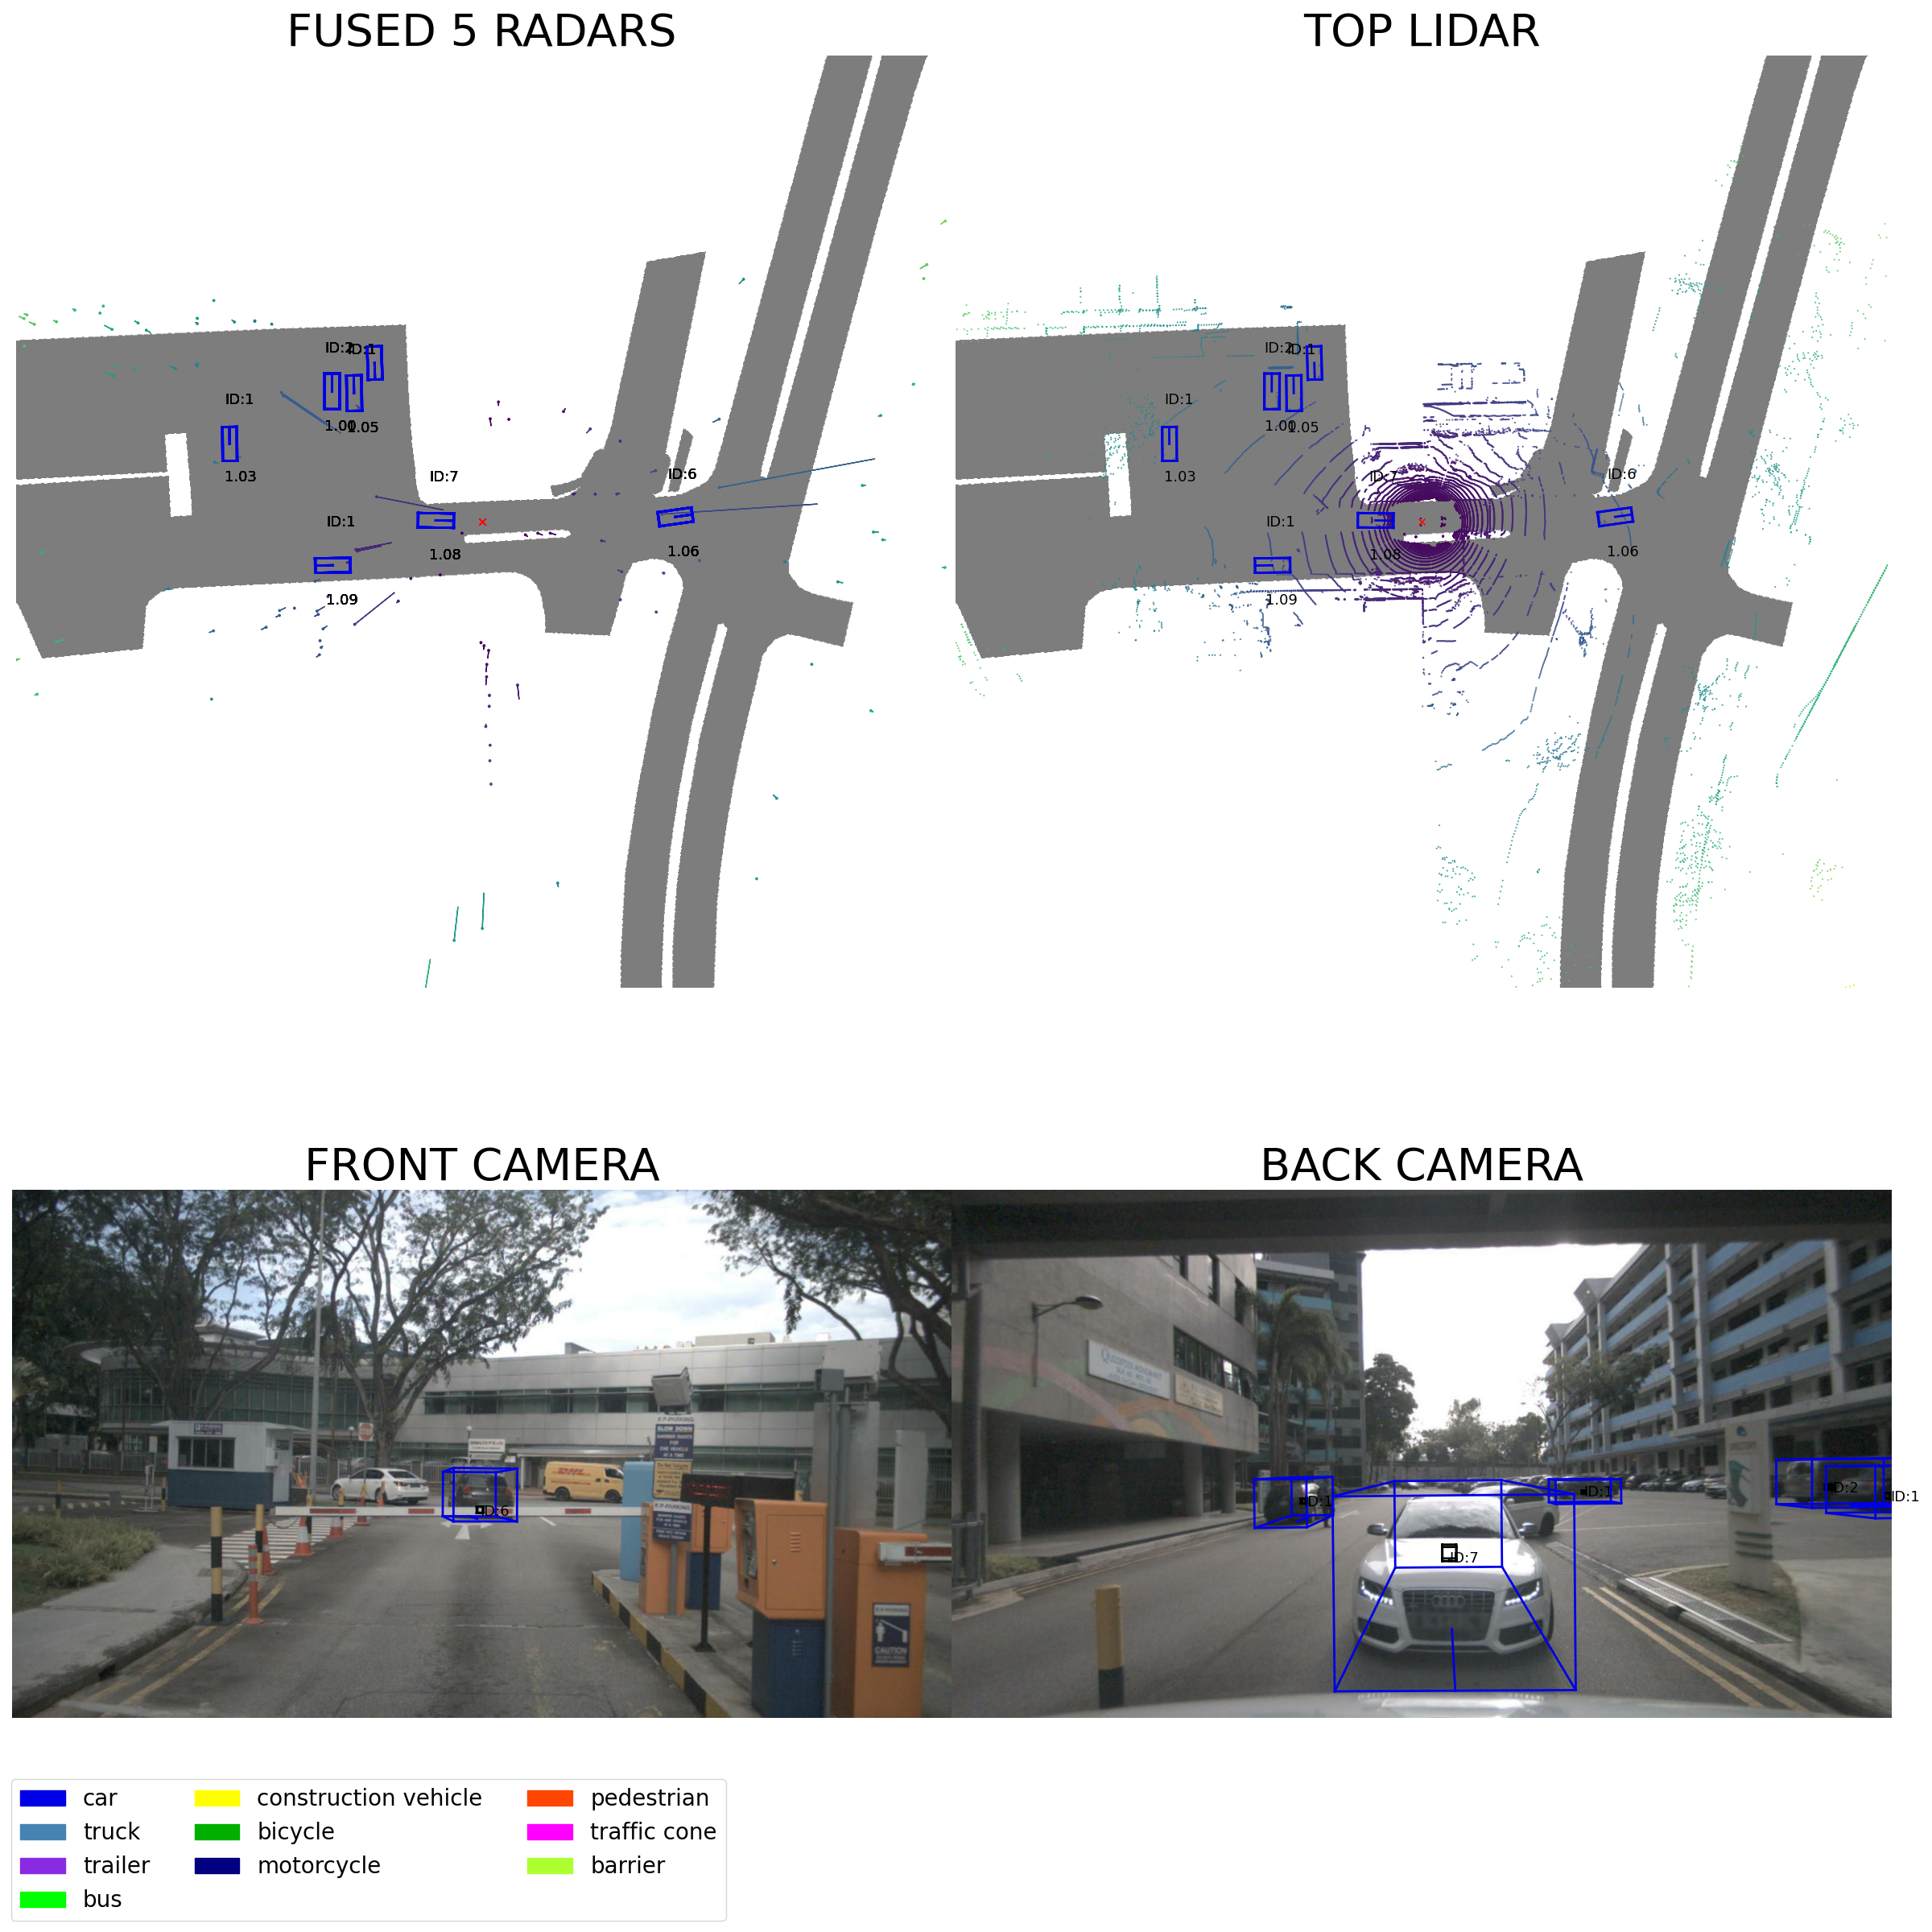
\includegraphics[width=0.4\linewidth]{demo/19.png}
    \end{figure}
\end{frame}
\begin{frame}{Demo}
    \begin{figure}
        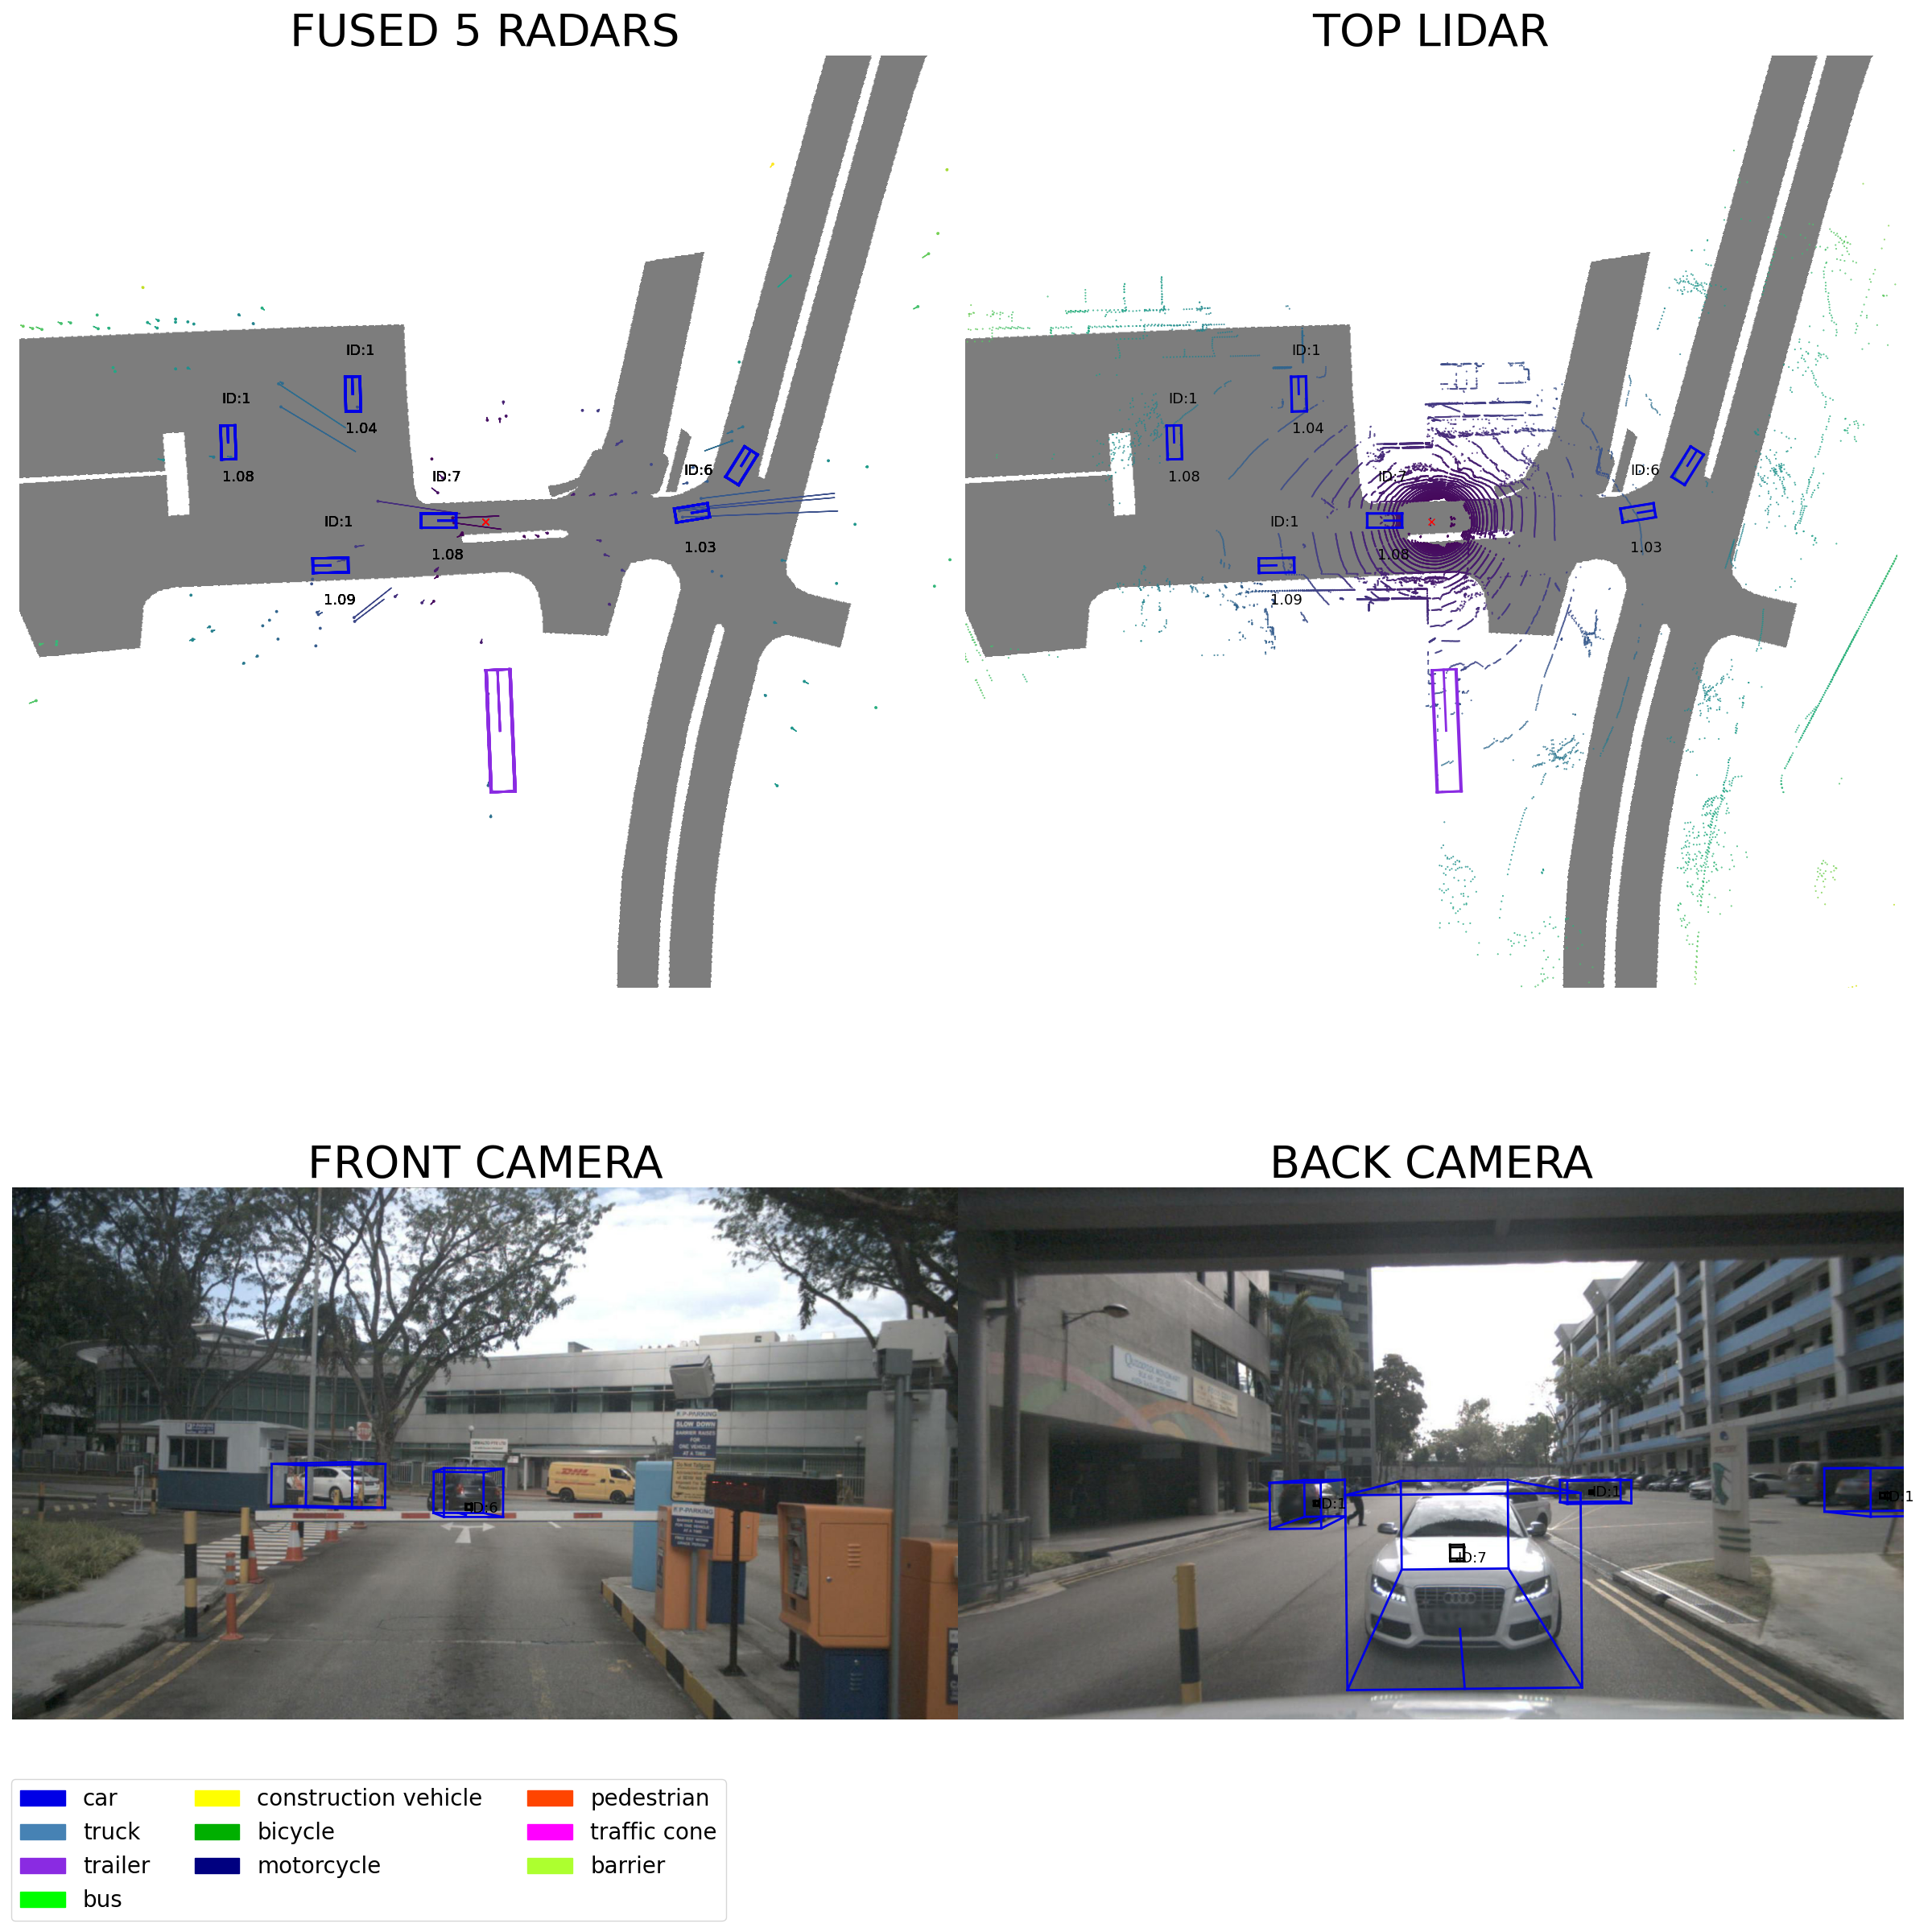
\includegraphics[width=0.4\linewidth]{demo/20.png}
    \end{figure}
\end{frame}
\begin{frame}{Demo}
    \begin{figure}
        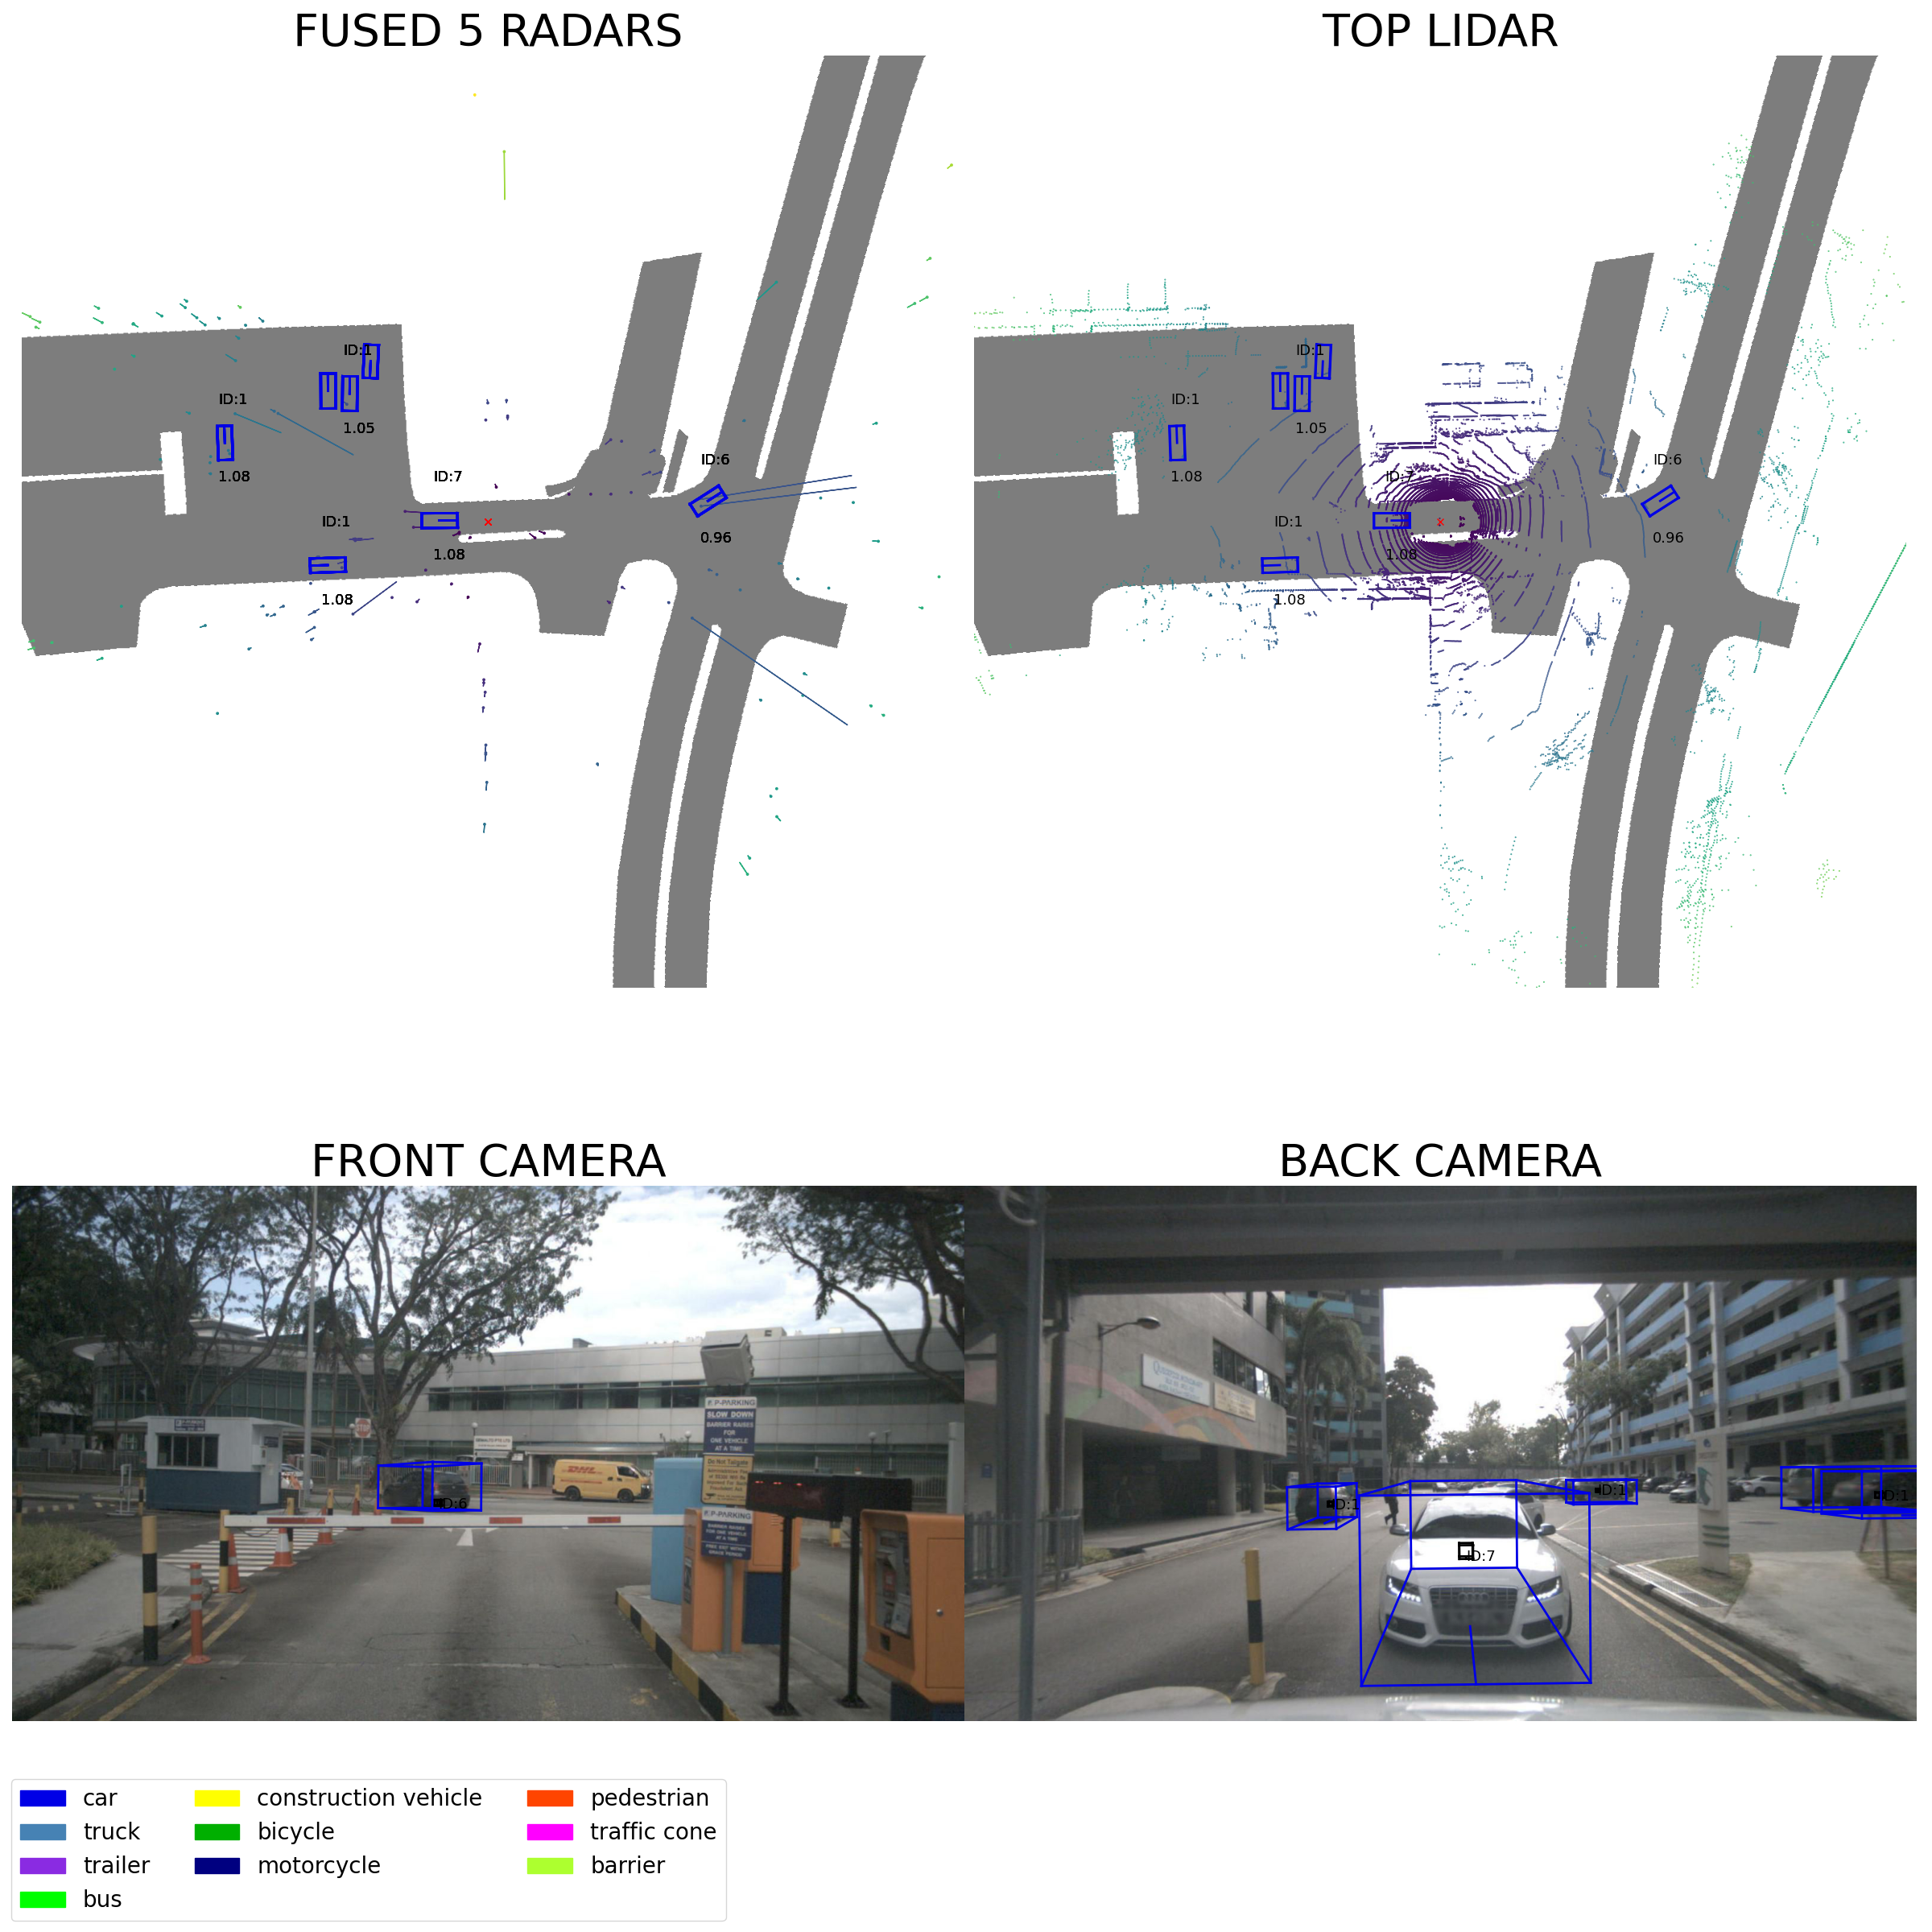
\includegraphics[width=0.4\linewidth]{demo/21.png}
    \end{figure}
\end{frame}
\begin{frame}{Demo}
    \begin{figure}
        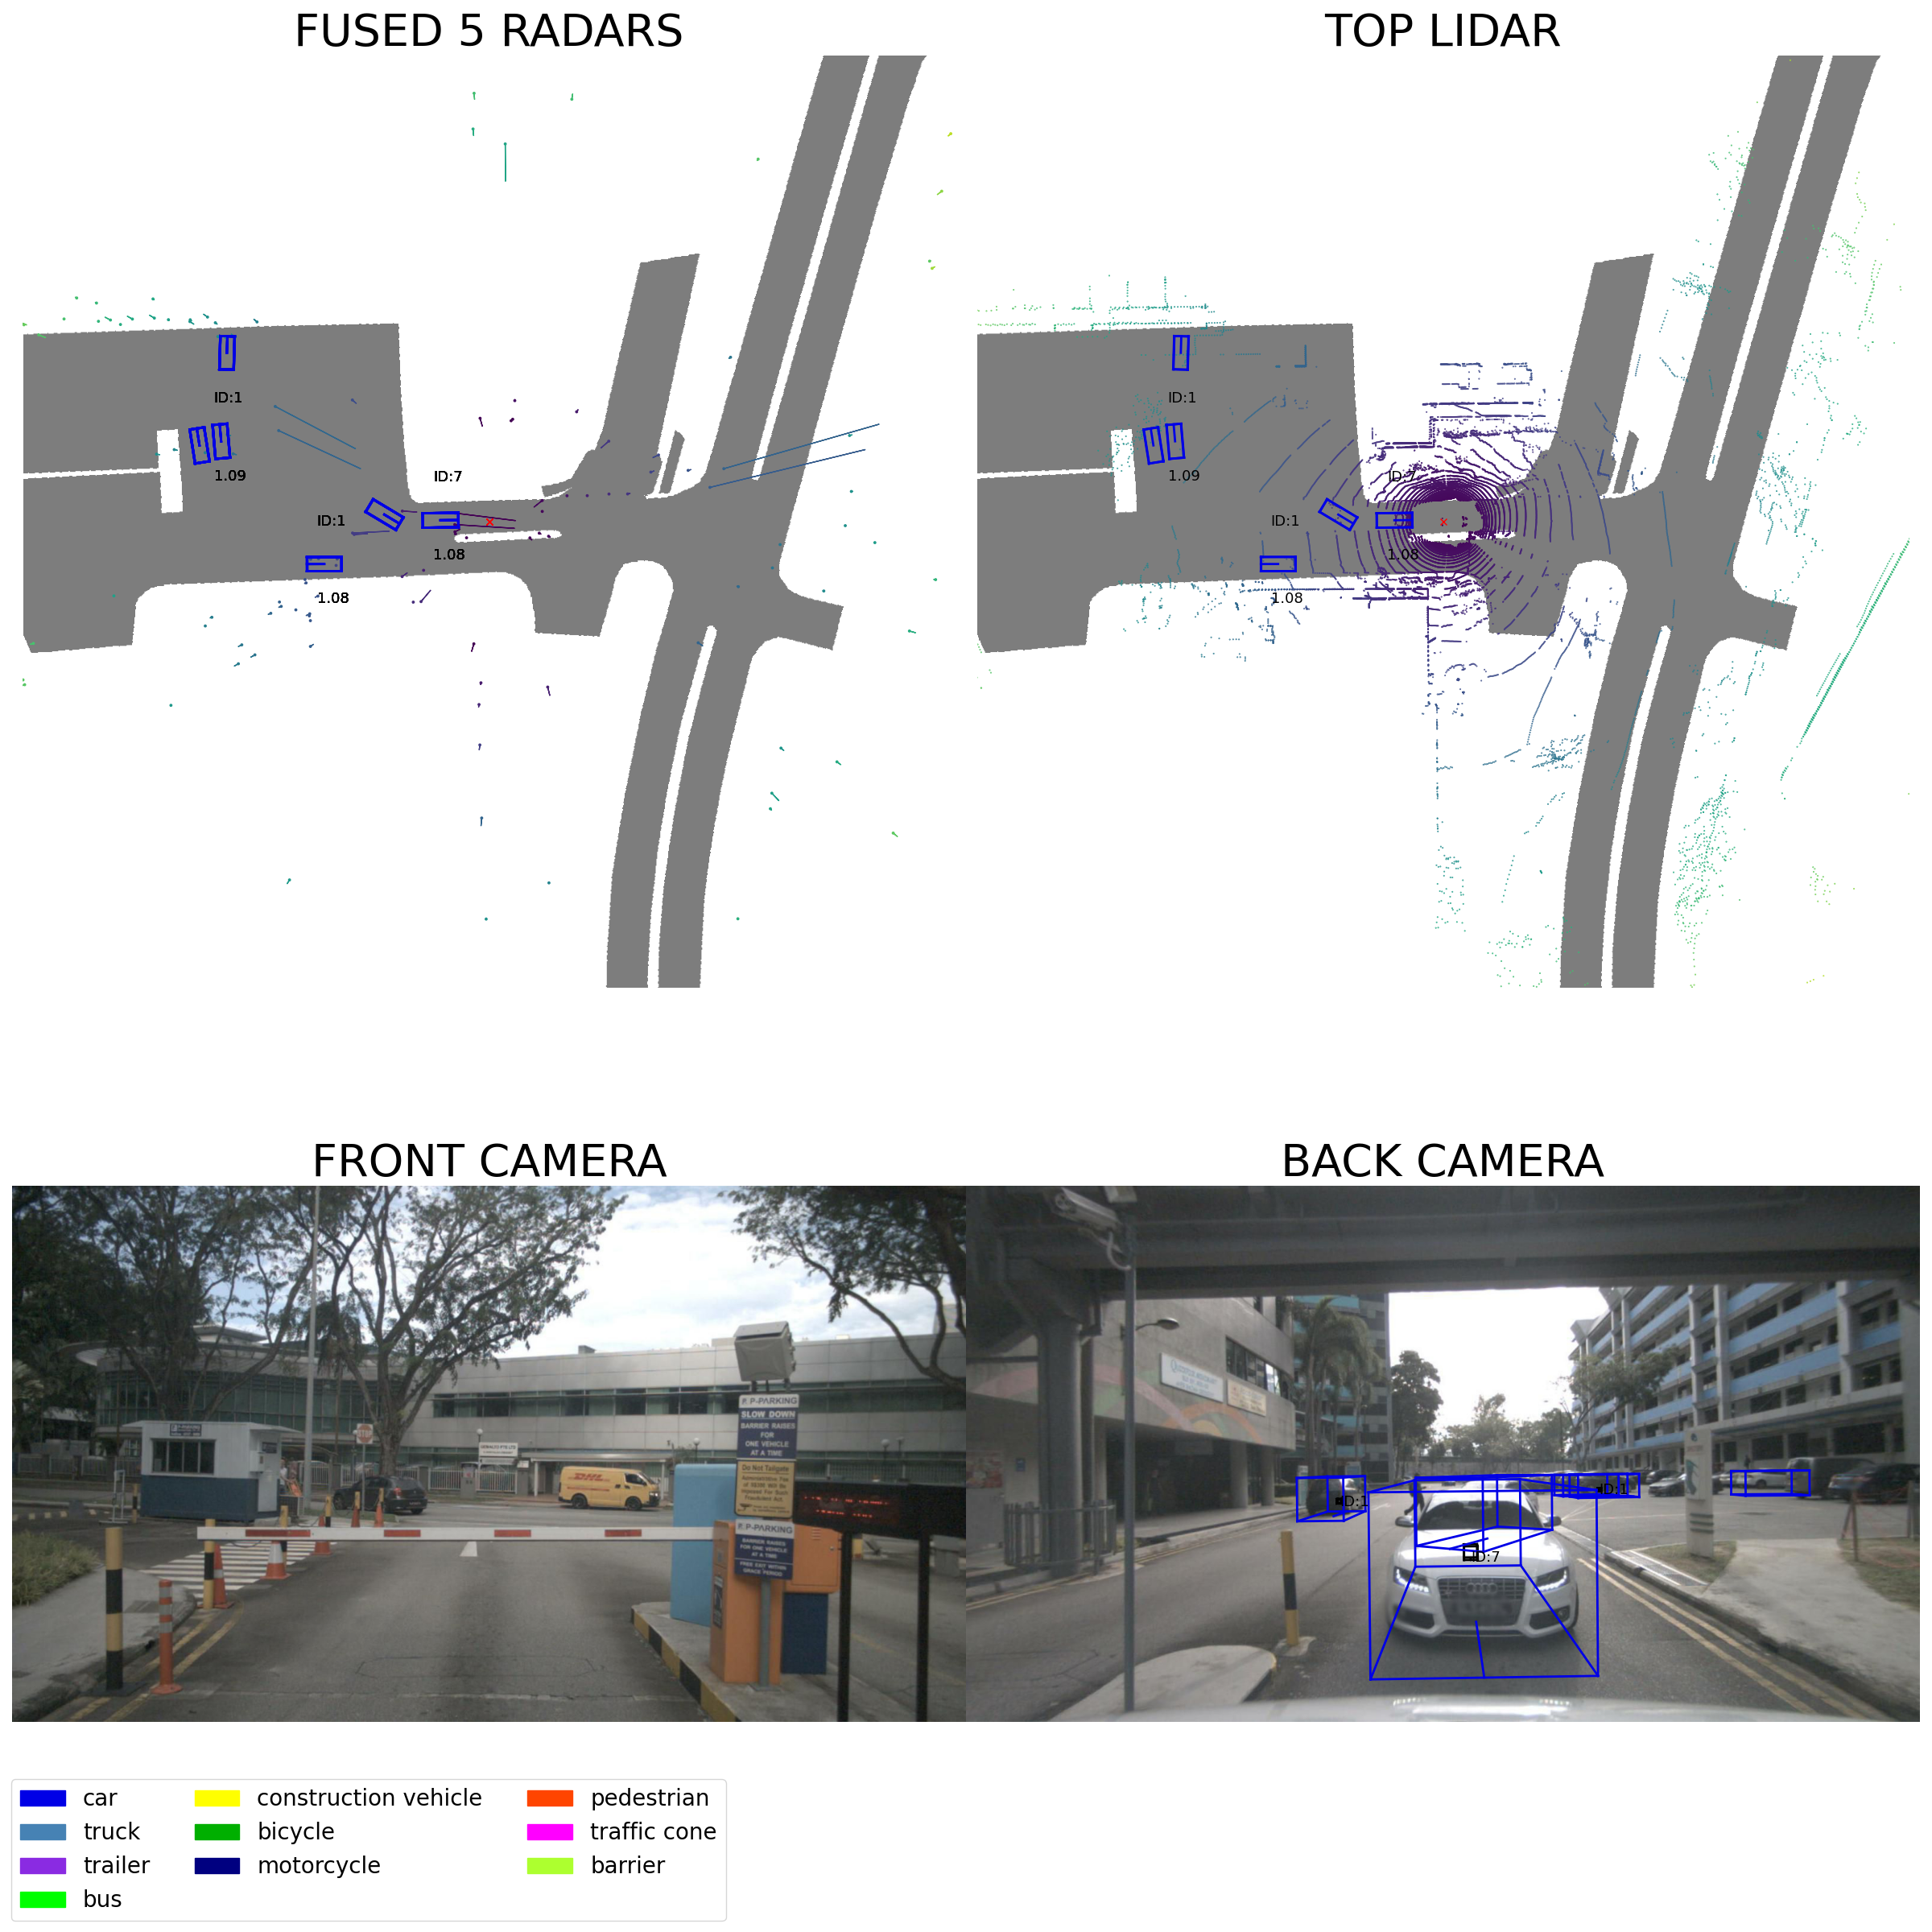
\includegraphics[width=0.4\linewidth]{demo/22.png}
    \end{figure}
\end{frame}
\begin{frame}{Demo}
    \begin{figure}
        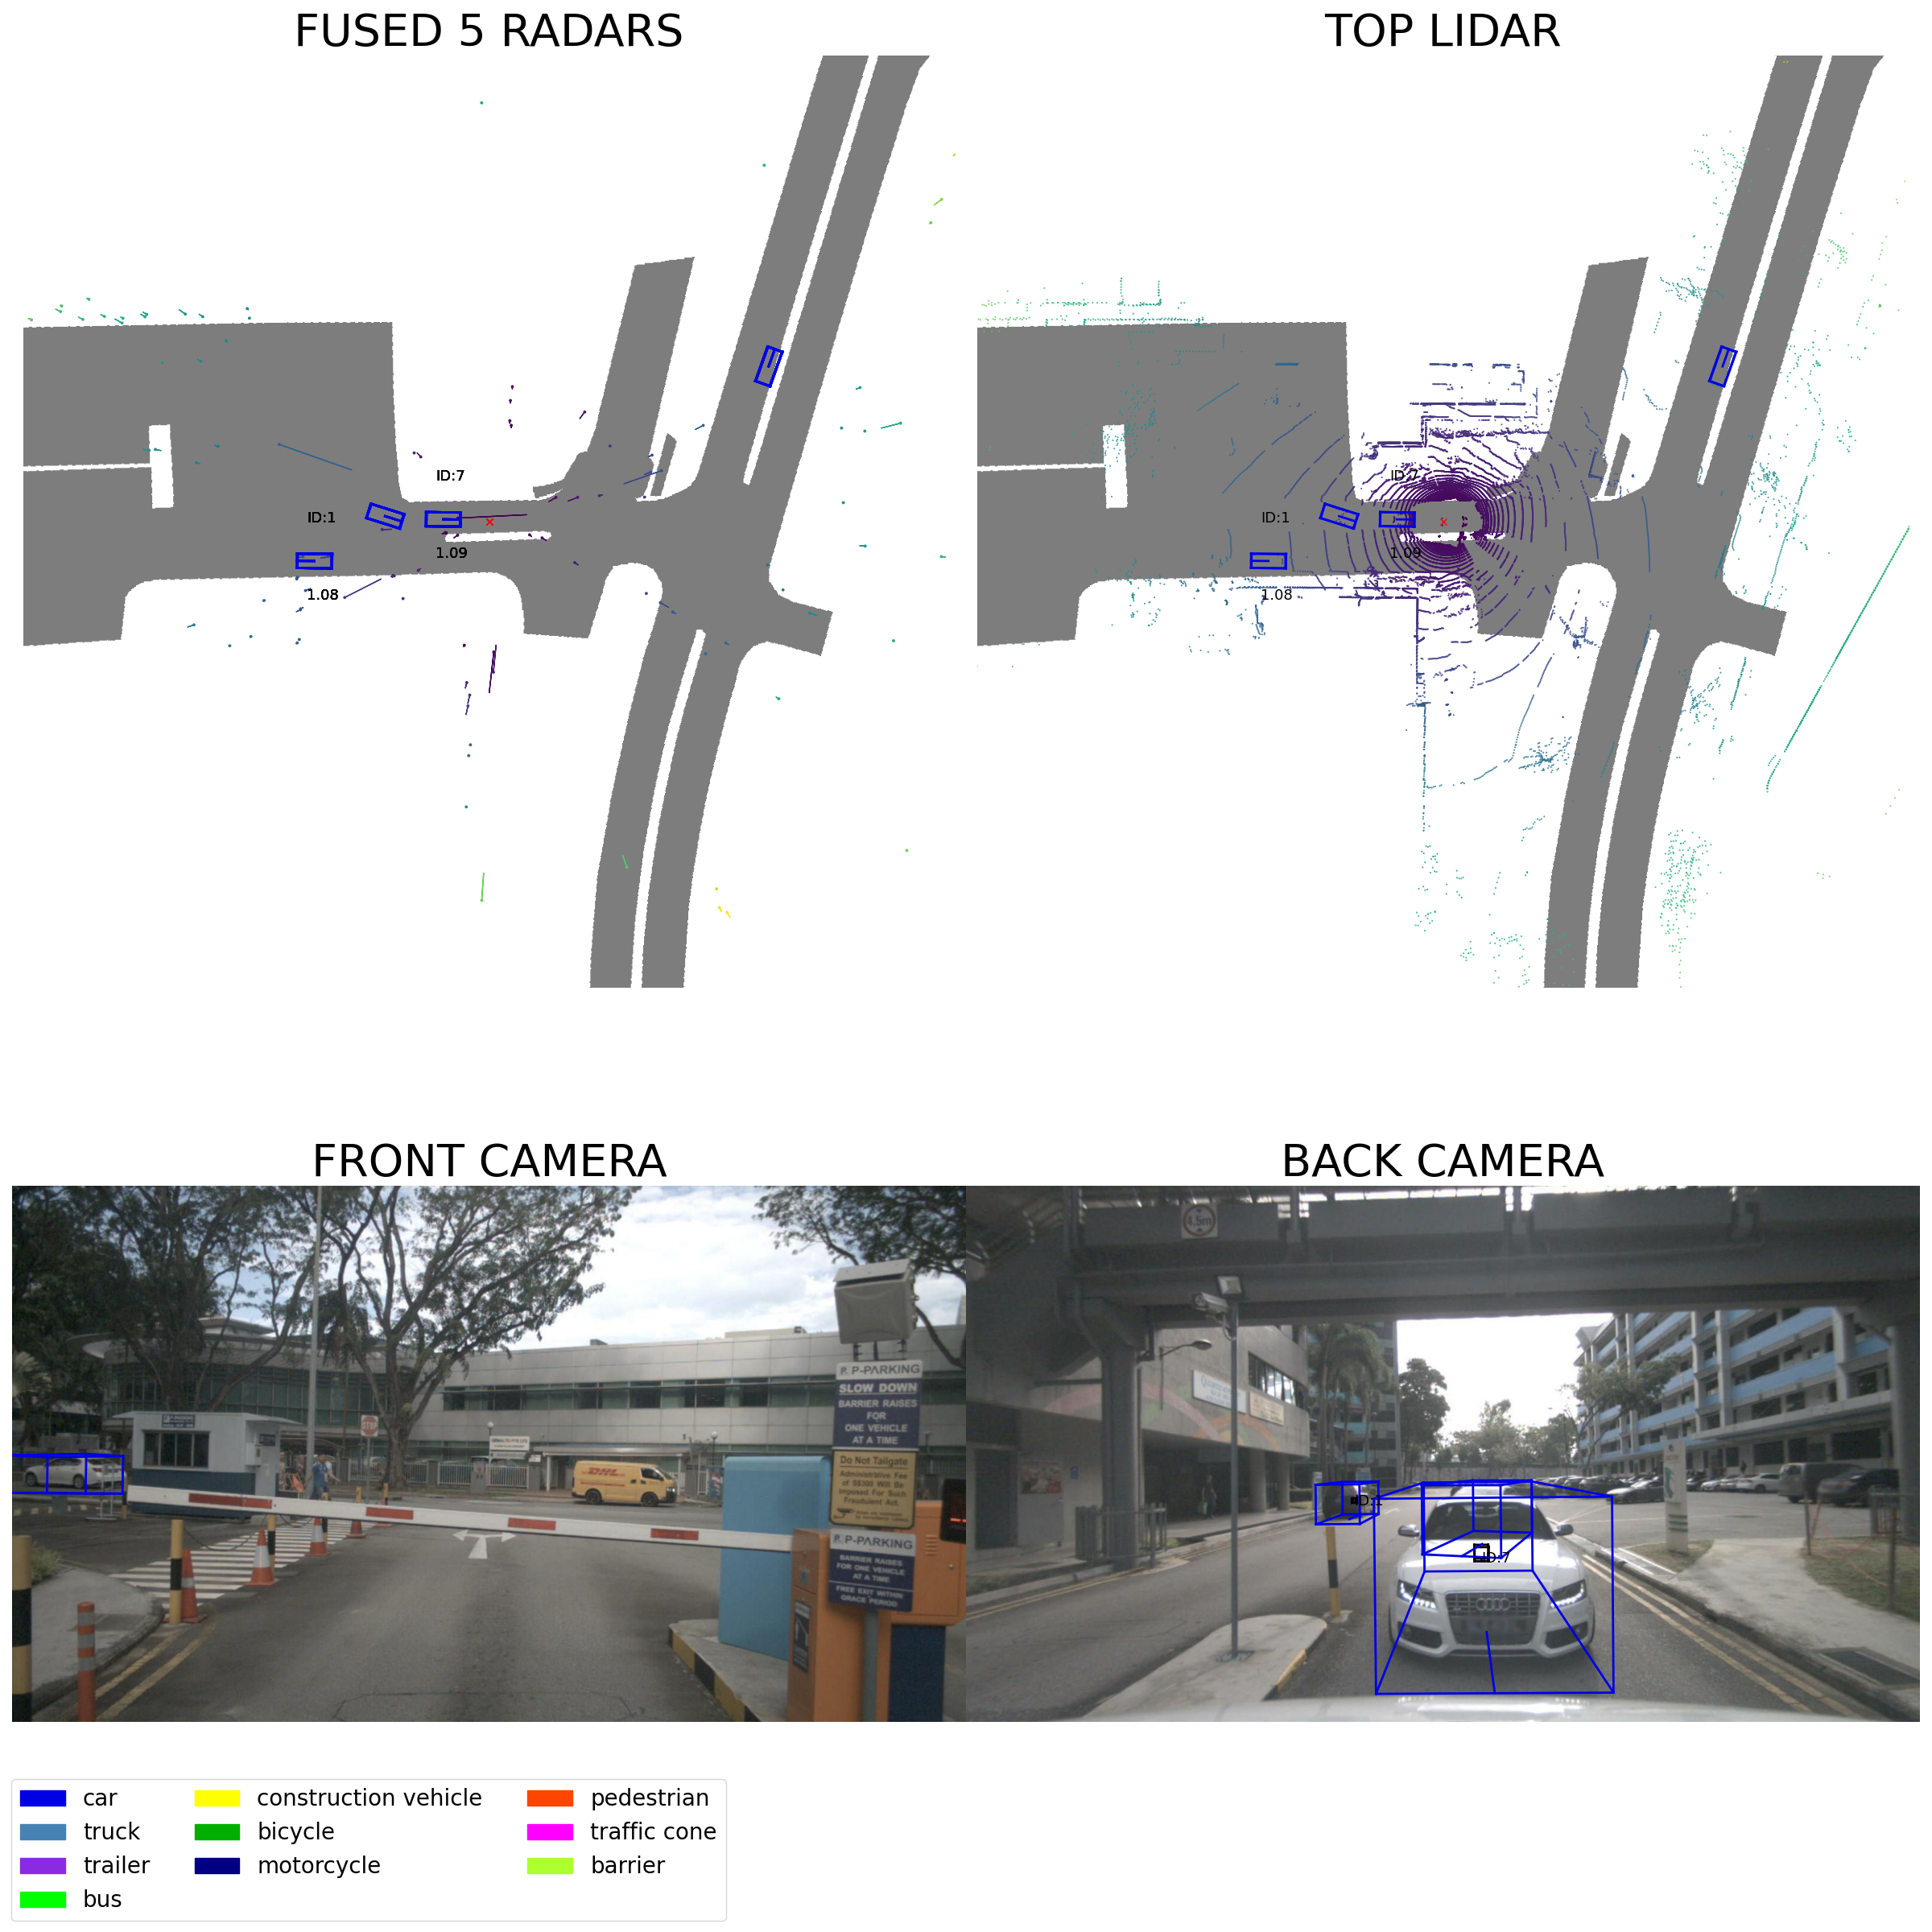
\includegraphics[width=0.4\linewidth]{demo/24.png}
    \end{figure}
\end{frame}
\begin{frame}{Demo}
    \begin{figure}
        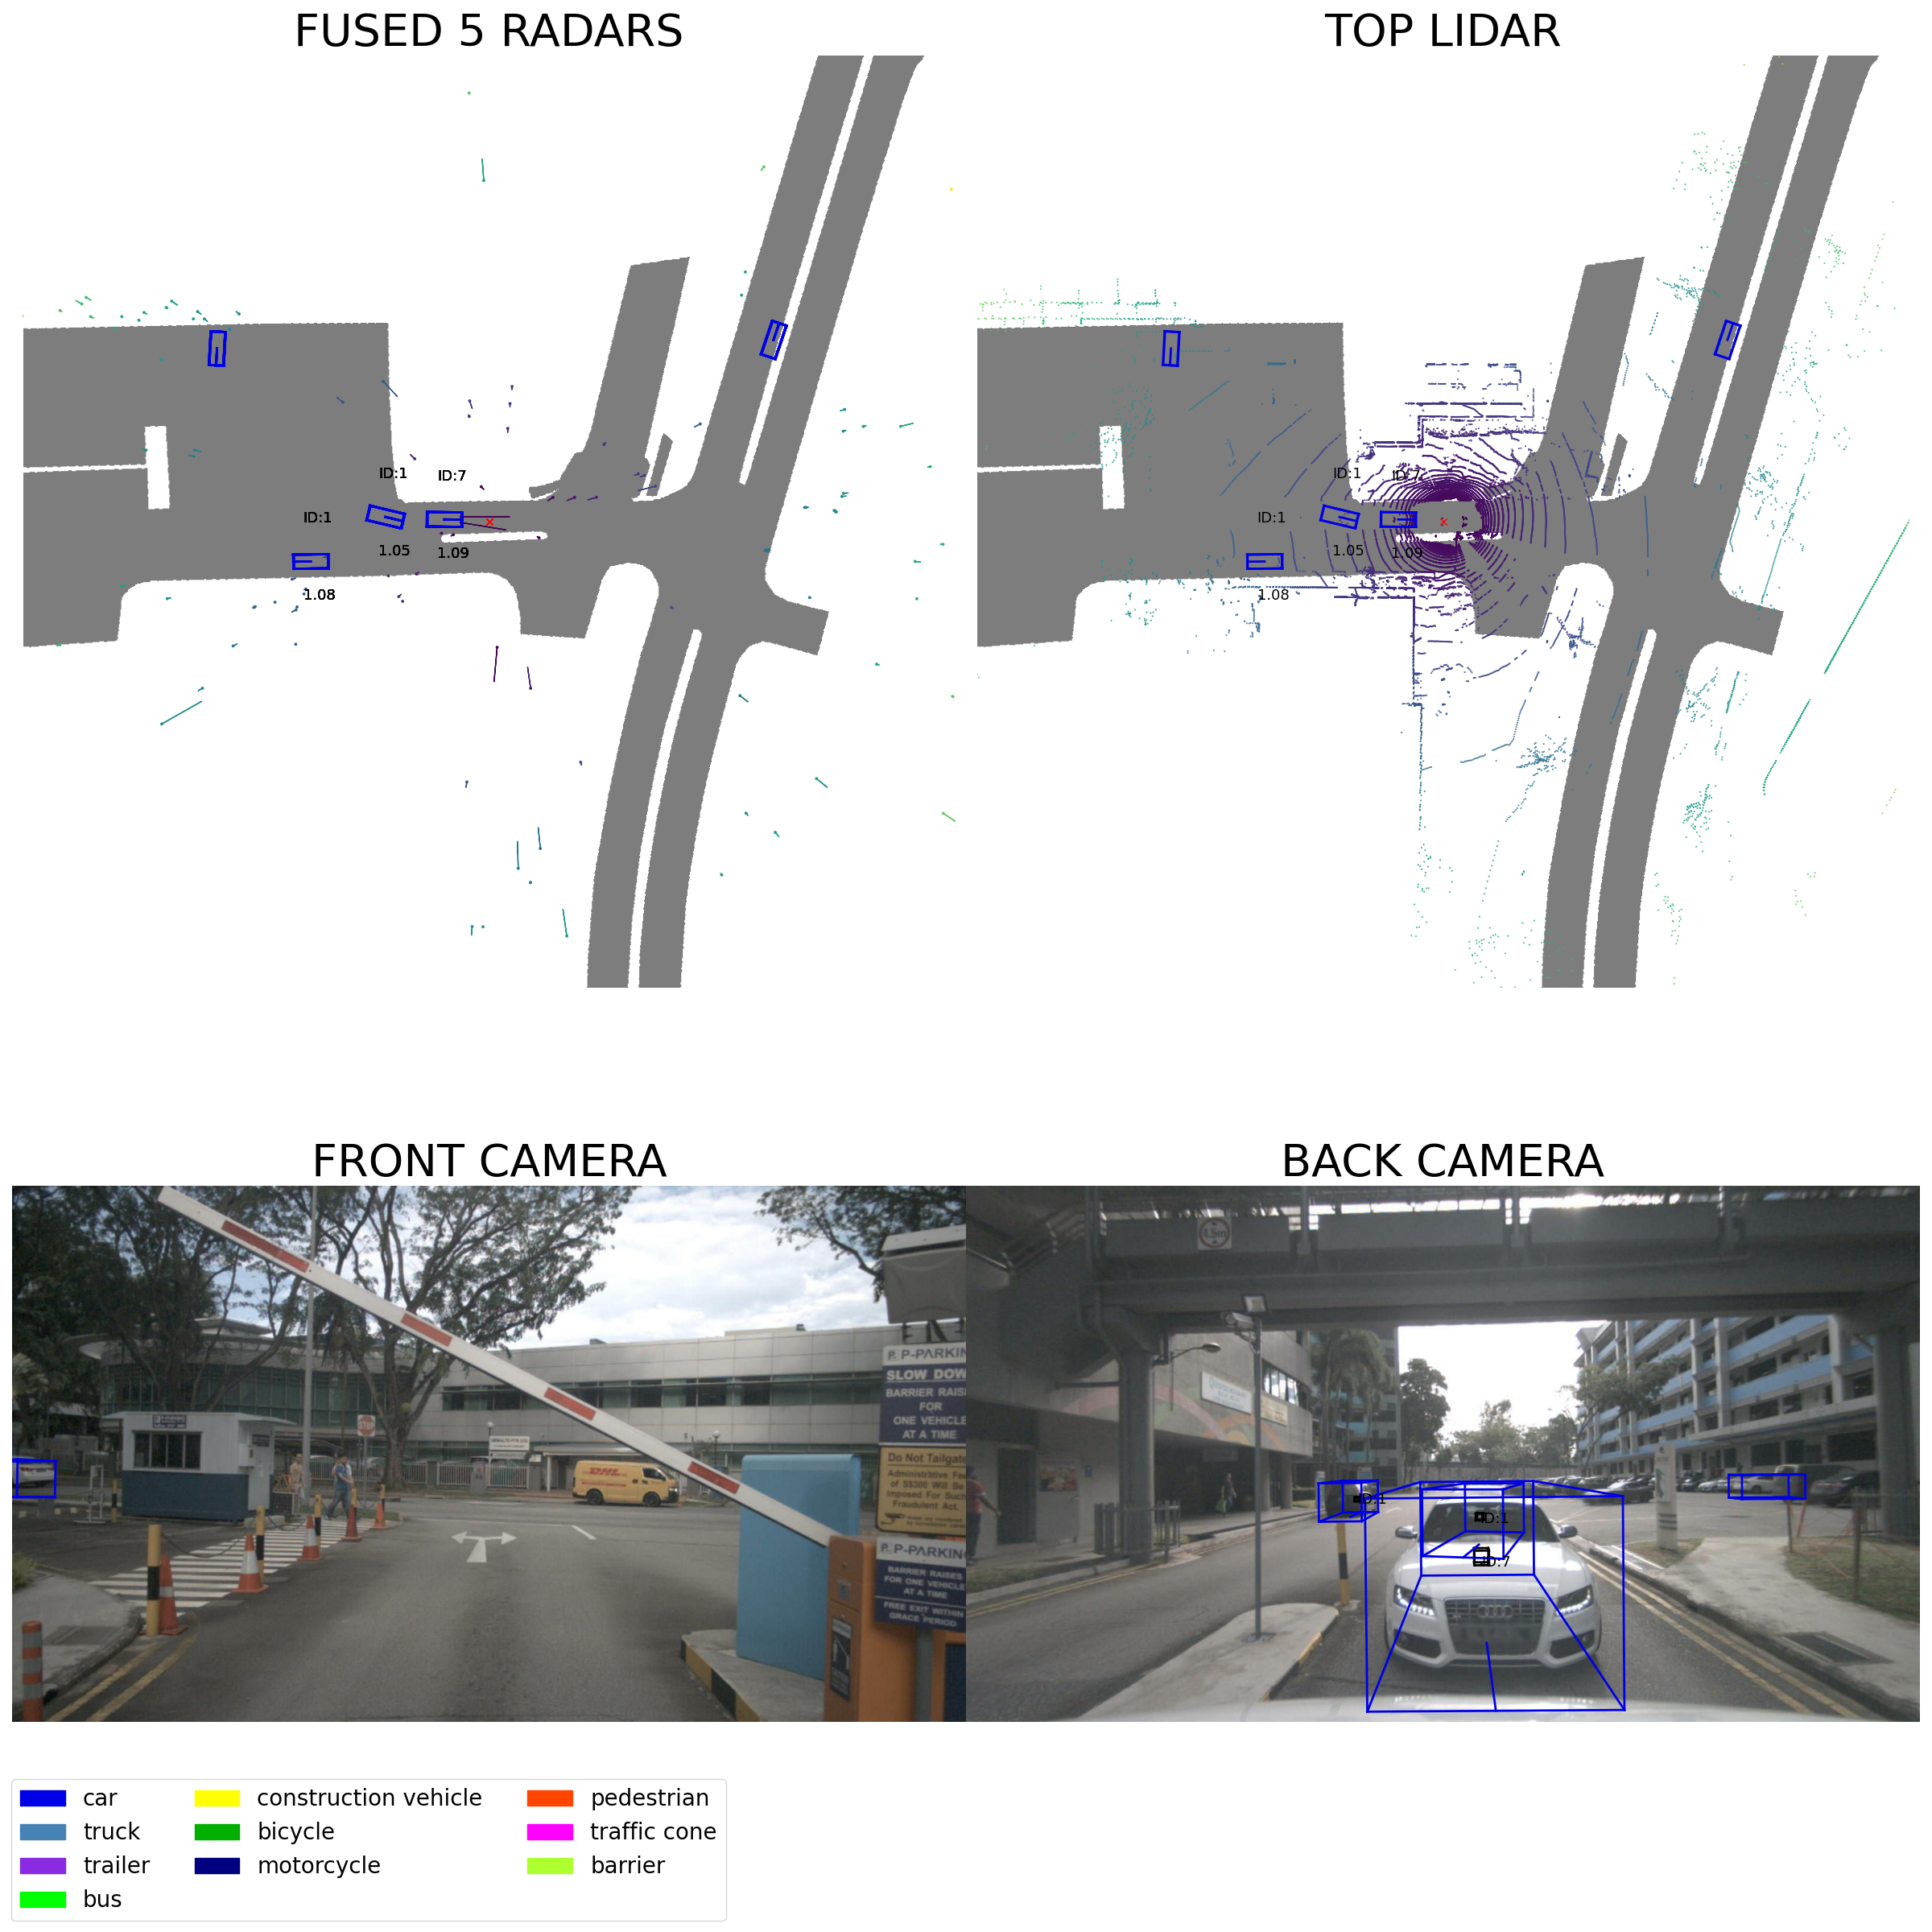
\includegraphics[width=0.4\linewidth]{demo/25.png}
    \end{figure}
\end{frame}
\begin{frame}{Demo}
    \begin{figure}
        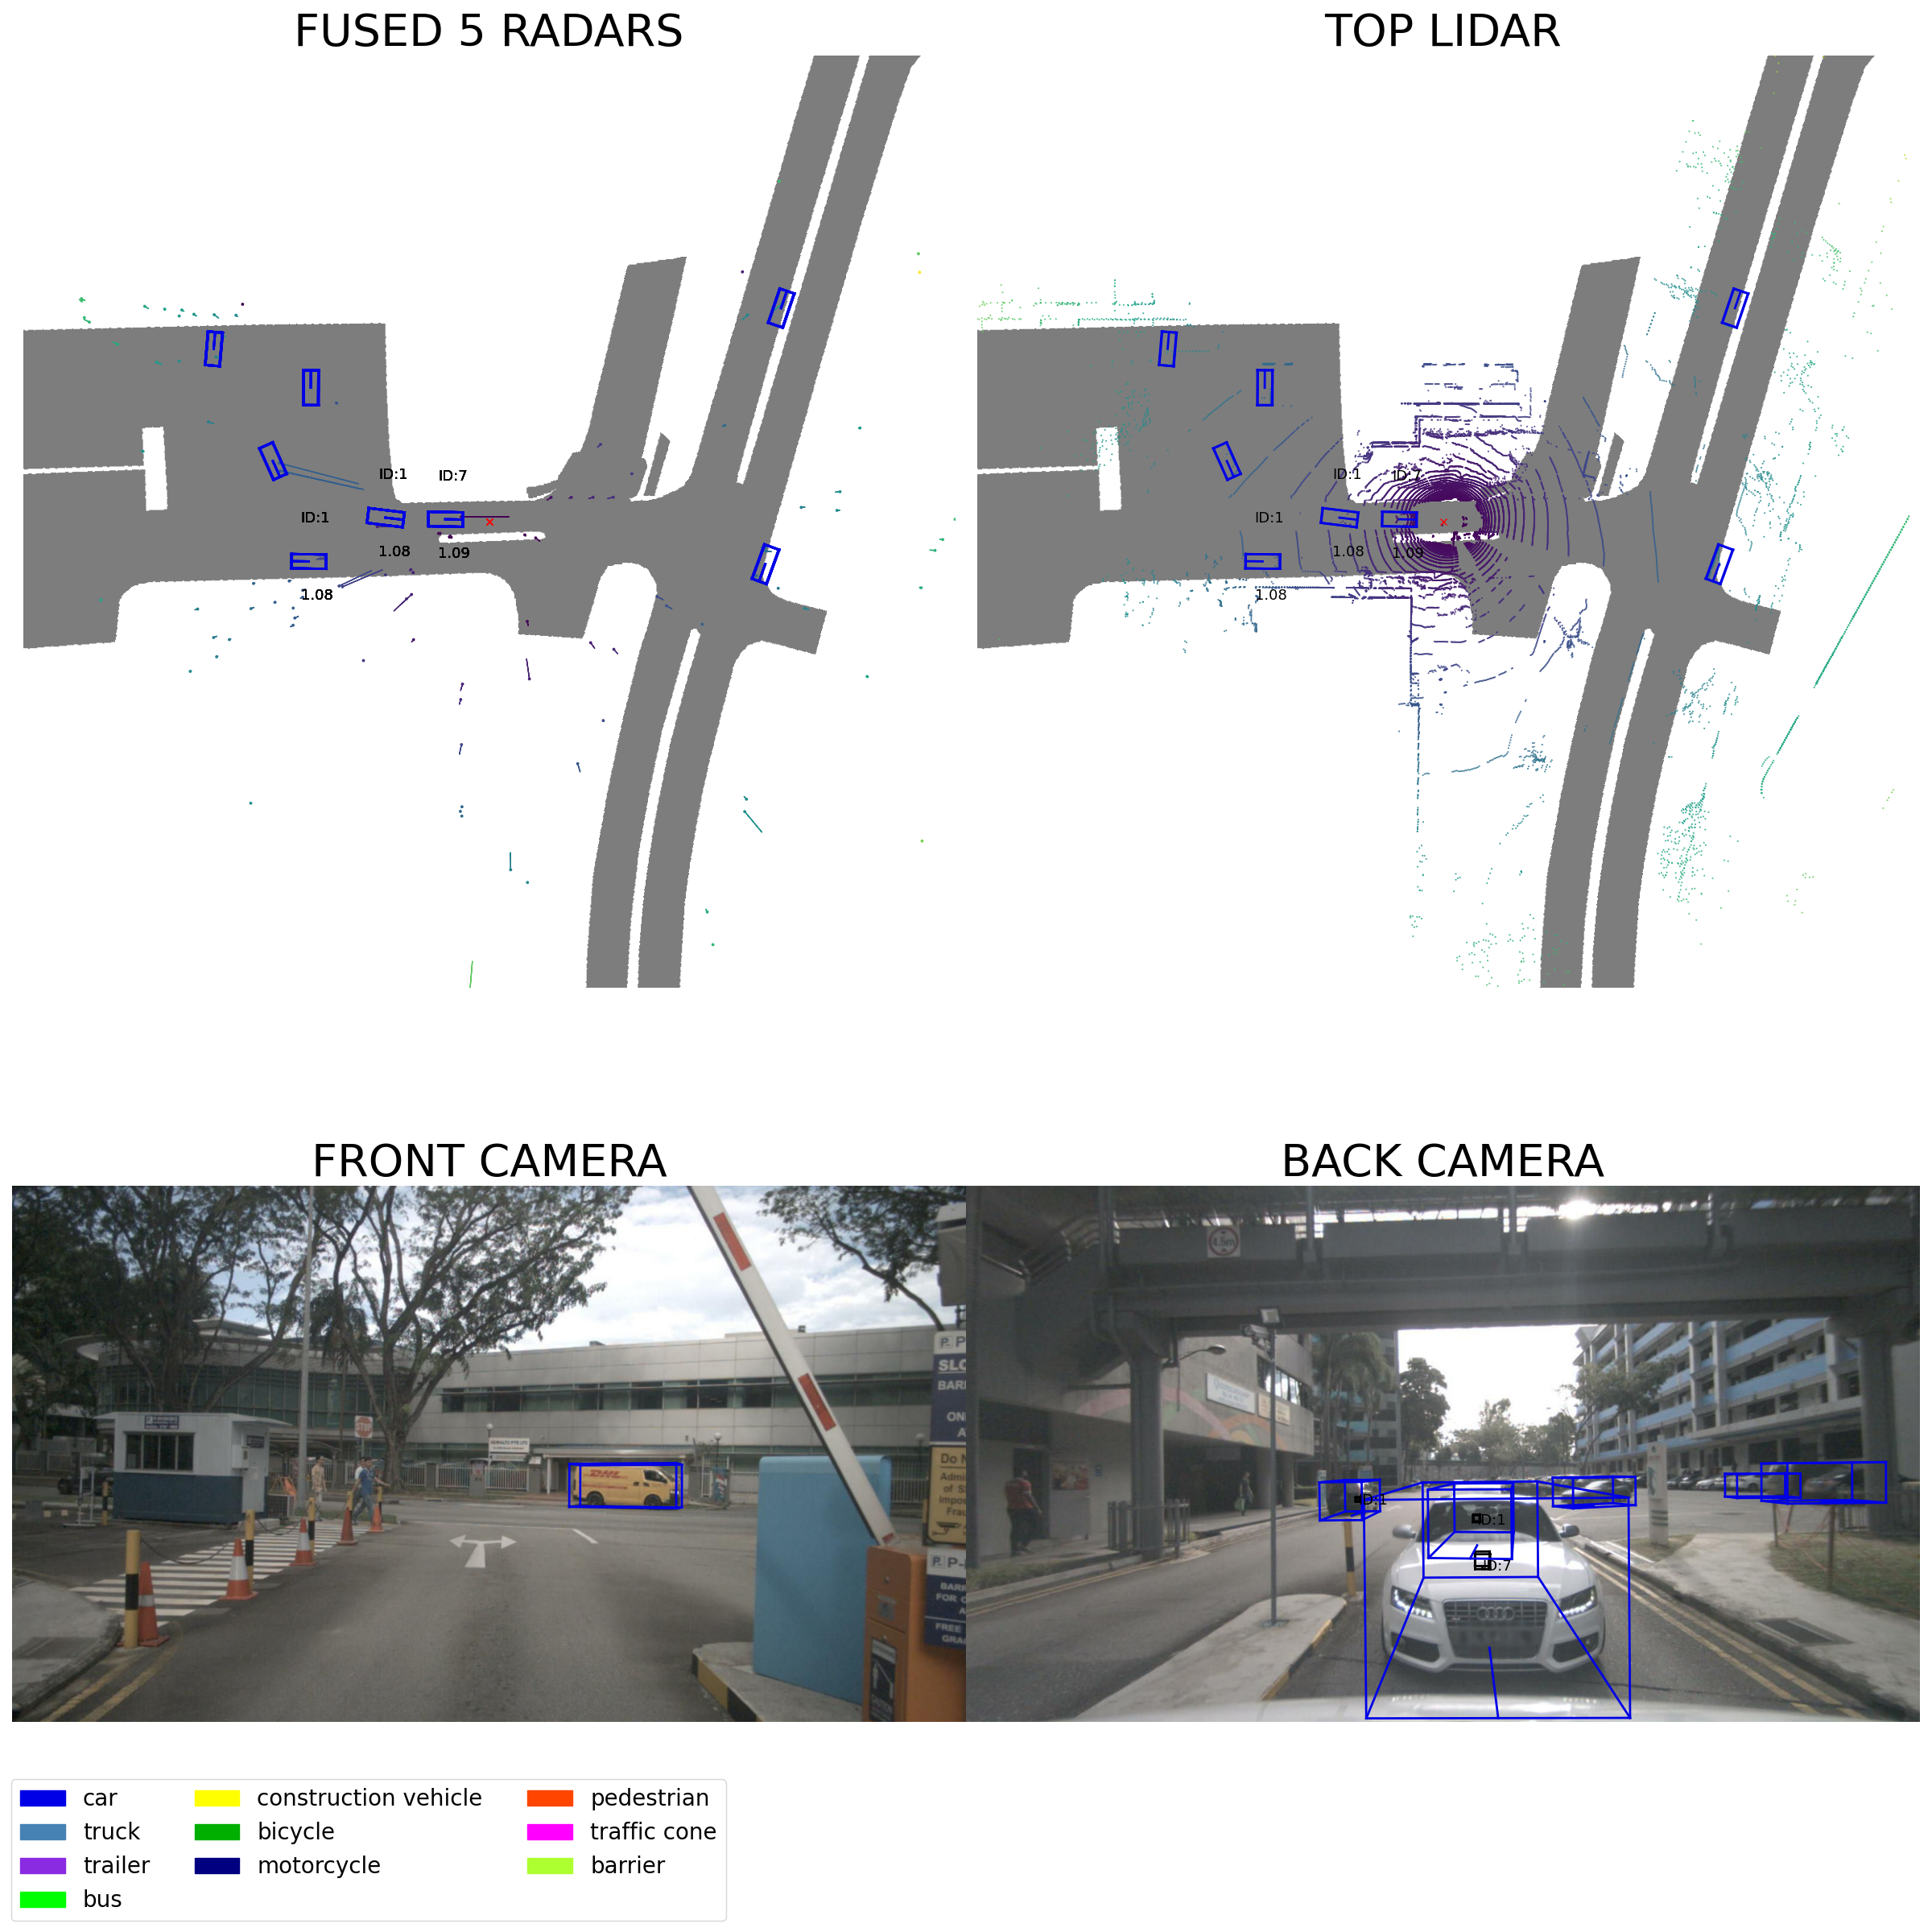
\includegraphics[width=0.4\linewidth]{demo/26.png}
    \end{figure}
\end{frame}
\begin{frame}{Demo}
    \begin{figure}
        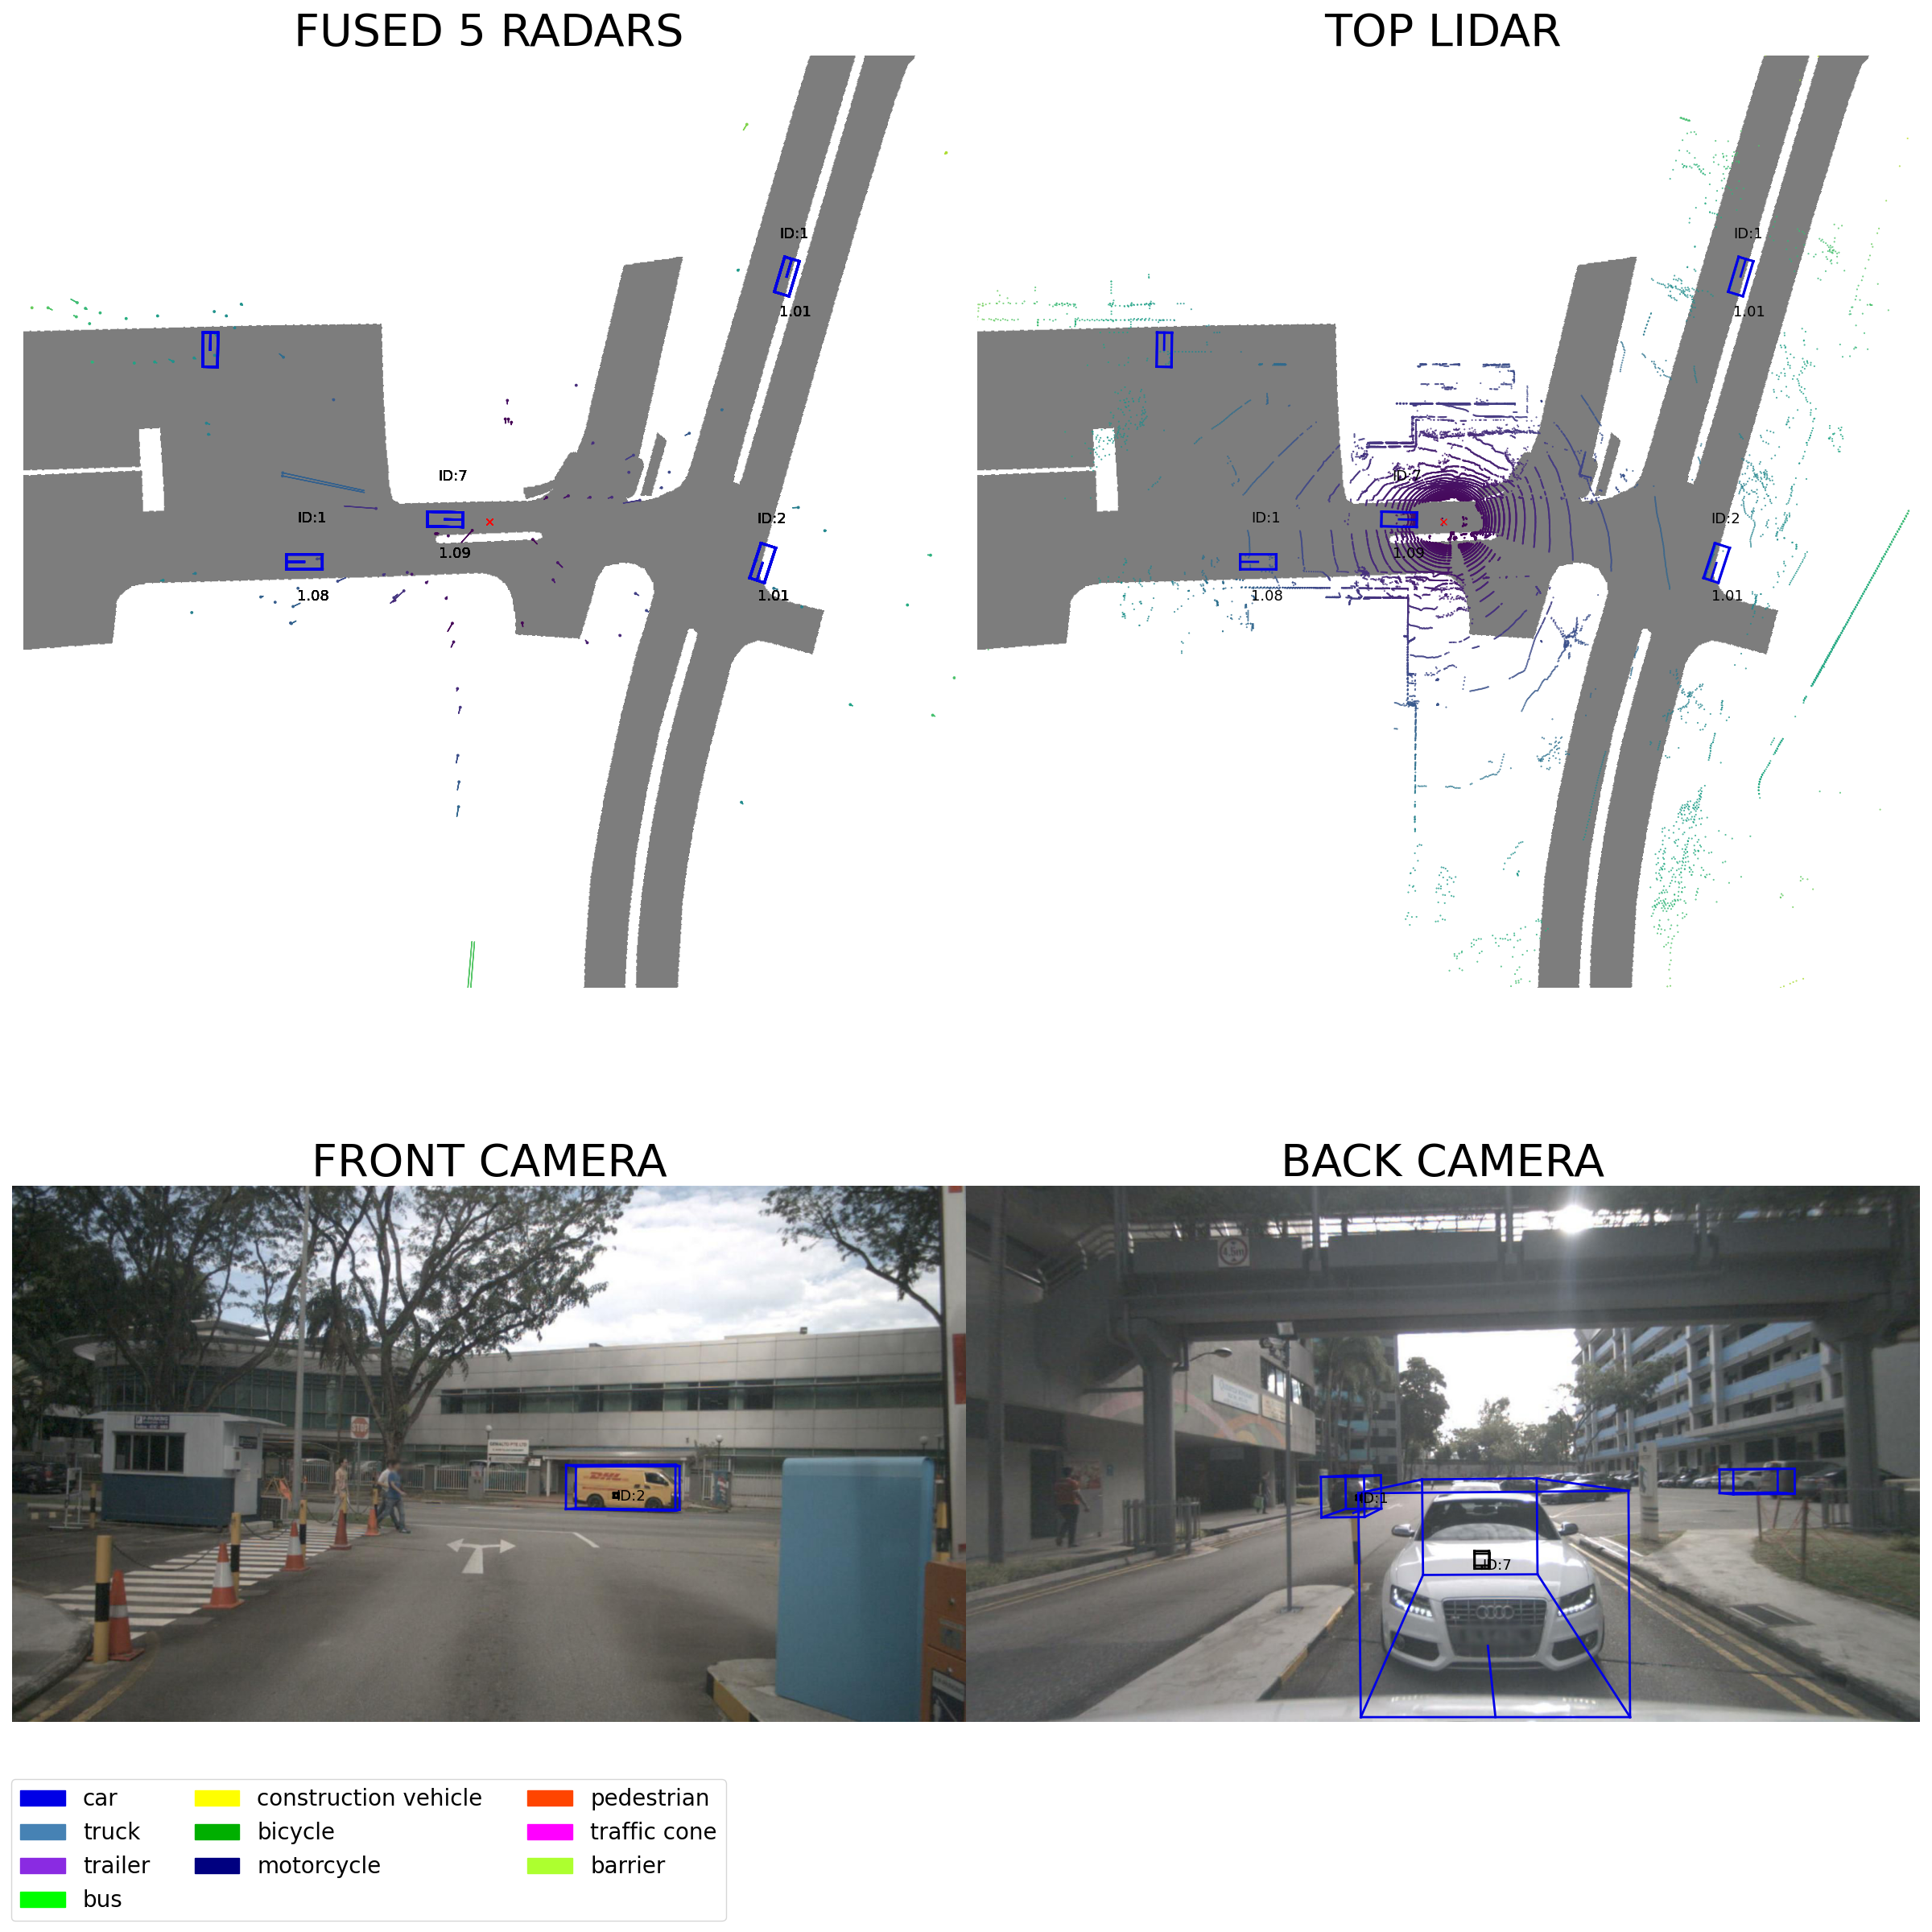
\includegraphics[width=0.4\linewidth]{demo/27.png}
    \end{figure}
\end{frame}

\begin{frame}{Problems to be solved}
    \begin{itemize}
        \item{birth}
    \end{itemize}
\end{frame}

\begin{frame}{PMBM birth Implementation}
    1. track management before poisson
    2. how to generate Bernoulli directly
    \begin{block}{}
    So unlike a standard PMBM filter, we incorporate the detection confidence score into the update step 
    of \textbf{objects detected for the first time}. 
    For detections with confidence scores larger than a threshold, 
    we generate a potential new target by adding \textbf{a new Bernoulli process}, 
    and plug the negative logarithm weight in the right m × m blocks diagonal in cost matrix L 
    discussed in Section IV-C. For detections with lower confidence score, 
    since we are not certain about their existences and require more evidences from the future, 
    an undetected track with PPP density is generated for each of them.
    \href{https://www.researchgate.net/publication/355428771_3D_Multi-Object_Tracking_using_Random_Finite_Set-based_Multiple_Measurement_Models_Filtering_RFS-M_3_for_Autonomous_Vehicles}{\beamergotobutton{paper}}
    \end{block}
\end{frame}

\begin{frame}{PMBM birth Implementation}
    birth with measurement + additive noise
    \begin{block}{}
    Add new Gaussian to the mixture (which represent the poisson intensity). This birth process is driven by
    measurements. Each measurement induce 3 birth of the same class by adding noise (uniformly distributed)
    \href{https://github.com/quan-dao/pmbm-filter/blob/5cdf8b31665f1a7008afa963c1ab7c3b048b5856/poisson.py}{\beamergotobutton{repository}}
    \end{block}
    \begin{figure}
        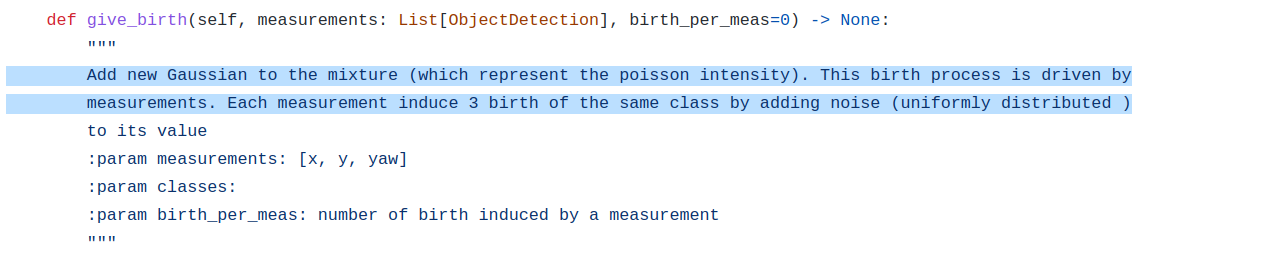
\includegraphics[width=0.9\linewidth]{pmbm/1.png}
    \end{figure}
\end{frame}

\begin{frame}{Research Plan}
    \begin{itemize}
        \item{Systematic Analysis over the mini dataset. Mini dataset is easier to evaluate. The test set takes around 1h to just do the evaluation.}
        \item{find out the best parameters}
        \item{implement that parameters for testset}
    \end{itemize}
\end{frame}

\begin{frame}{Literature Review}
\begin{block}{Measurement-Track association NOT a performance constraint for Lidar based MOT}
    \textbf{THE RESEARCH DIRECTION NEED TO BE REEVALUATED}
\end{block}
\end{frame}
\end{document}